%%%%%%%%%%%%%%%%%%%%%%%%%%%%%%%%%%%%%%%%%%%%%%%%%%%%%%%%%%%%%%%%%%
%%%%%%%% ICML 2017 EXAMPLE LATEX SUBMISSION FILE %%%%%%%%%%%%%%%%%
%%%%%%%%%%%%%%%%%%%%%%%%%%%%%%%%%%%%%%%%%%%%%%%%%%%%%%%%%%%%%%%%%%

% Use the following line _only_ if you're still using LaTeX 2.09.
%\documentstyle[icml2017,epsf,natbib]{article}
% If you rely on Latex2e packages, like most moden people use this:
\documentclass{article}

% use Times
\usepackage{times}
% For figures
\usepackage{graphicx} % more modern
%\usepackage{epsfig} % less modern
\usepackage{subfigure} 

% For citations
\usepackage{natbib}

% For algorithms
\usepackage{algorithm}
\usepackage{algorithmic}

% As of 2011, we use the hyperref package to produce hyperlinks in the
% resulting PDF.  If this breaks your system, please commend out the
% following usepackage line and replace \usepackage{icml2017} with
% \usepackage[nohyperref]{icml2017} above.
\usepackage{hyperref}

% Packages hyperref and algorithmic misbehave sometimes.  We can fix
% this with the following command.
\newcommand{\theHalgorithm}{\arabic{algorithm}}

% Employ the following version of the ``usepackage'' statement for
% submitting the draft version of the paper for review.  This will set
% the note in the first column to ``Under review.  Do not distribute.''
\usepackage{icml2017} 

% Employ this version of the ``usepackage'' statement after the paper has
% been accepted, when creating the final version.  This will set the
% note in the first column to ``Proceedings of the...''
%\usepackage[accepted]{icml2017}
\usepackage{fullpage}
\usepackage{amsthm}
\usepackage{amssymb}
\newtheorem{theorem}{Theorem}[section]
\newtheorem{lemma}[theorem]{Lemma}
\newtheorem{fact}[theorem]{Fact}
\newtheorem{proposition}[theorem]{Proposition}
\newtheorem{observation}[theorem]{Observation}
\newtheorem{corollary}[theorem]{Corollary}
\newtheorem{remark}[theorem]{Remark}
\newtheorem{conjecture}[theorem]{Conjecture}
\newtheorem{definition}[theorem]{Definition}
\newtheorem{claim}[theorem]{Claim}
\newtheorem{assumption}{Assumption}

\usepackage{amsmath}
\usepackage{thmtools, thm-restate}
\usepackage{multirow}
\usepackage{tabularx}
\usepackage{colortbl}
\usepackage{color}
\usepackage[small]{caption}
%\usepackage[ruled,vlined]{algorithm2e}


%%%%%%%%%%%%% Macros %%%%%%%%%%%%% 
\newcommand{\llabel}[1]{\label{#1}}
\newcommand{\heading}[1]{{\bf #1}}

\newcommand{\zo}{\{0,1\}}
\newcommand{\mzo}{\{-1,+1\}}
\newcommand{\F}{{\mathbb{F}}}
\newcommand{\N}{{\mathbb{N}}}
\newcommand{\Z}{{\mathbb{Z}}}
\newcommand{\R}{{\mathbb{R}}}
\newcommand{\C}{{\mathbb{C}}}
\newcommand{\eps}{\epsilon}
\newcommand{\beq}{\begin{eqnarray}}
\newcommand{\eeq}{\end{eqnarray}}
\newcommand{\tO}{\tilde{O}}
\newcommand{\bt}{\tilde{b}}
\newcommand{\vb}{{\bar b}}
\newcommand{\sign}{\text{sign}}
\newcommand{\T}{T}
\newcommand{\ip}[1]{\langle #1 \rangle}
\DeclareMathOperator{\Tr}{Tr}

\newcommand{\Vol}{\mathop\mathrm{Vol}\nolimits}
\newcommand{\Const}{\mathop\mathrm{Const}\nolimits}
\DeclareMathOperator*{\expt}{\mathbb{E}}
\newcommand{\E}[2]{{\mathbb{E}_{#1}\left[#2\right]}}
\newcommand{\EE}[2]{{\expt_{#1}{#2}}}
\newcommand{\EX}{{\mathbb E}}
\newcommand{\Sur}{\mathop\mathrm{Sur}\nolimits}
\newcommand{\polylog}{\mathop\mathrm{polylog}\nolimits}
\newcommand{\xor}{\oplus}
\newcommand{\conj}[1]{{\overline {#1}}} %% conjugate
\newcommand{\pd}[2]{\frac{\partial#1}{\partial#2}}


\def\showauthornotes{1}

%%%%%%%%%%%%%% Use for definitions
\newcommand{\defeq}{\stackrel{\textup{def}}{=}}

%%%%%%%%%%%%%% Probability stuff
\DeclareMathOperator*{\pr}{\bf Pr}
\DeclareMathOperator*{\av}{\bf E}
\DeclareMathOperator*{\var}{\bf Var}

%%%%%%%%%%%%%% Matrix stuff
\newcommand{\tr}[1]{\mathop{\mbox{$\mathrm{Tr}$}}\left({#1}\right)}
\newcommand{\diag}[1]{{\bf Diag}\left({#1}\right)}

%% Notation for integers, natural numbers, reals, fractions, sets, cardinalities
%%and so on
\newcommand{\nfrac}[2]{\nicefrac{#1}{#2}}
\def\abs#1{\left| #1 \right|}
\newcommand{\norm}[1]{\ensuremath{\left\lVert #1 \right\rVert}}

\newcommand{\floor}[1]{\left\lfloor\, {#1}\,\right\rfloor}
\newcommand{\ceil}[1]{\left\lceil\, {#1}\,\right\rceil}

\newcommand{\pair}[1]{\left\langle{#1}\right\rangle} %for inner product

\newcommand\B{\{0,1\}}      % boolean alphabet  use in math mode
\newcommand\bz{\mathbb Z}
\newcommand\nat{\mathbb N}
\newcommand\rea{\mathbb R}
\newcommand\com{\mathbb{C}}
\newcommand\plusminus{\{\pm 1\}}
\newcommand\Bs{\{0,1\}^*}   % B star use in math mode

\newcommand{\V}[1]{\mathbf{#1}} % Used to denote bold commands
                                % e.g. vectors, matrices
\DeclareRobustCommand{\fracp}[2]{{#1 \overwithdelims()#2}}
\DeclareRobustCommand{\fracb}[2]{{#1 \overwithdelims[]#2}}
\newcommand{\marginlabel}[1]%
{\mbox{}\marginpar{\it{\raggedleft\hspace{0pt}#1}}}
\newcommand\card[1]{\left| #1 \right|} %cardinality of set S; usage \card{S}
\newcommand\set[1]{\left\{#1\right\}} %usage \set{1,2,3,,}
%\renewcommand\complement{\ensuremath{\mathsf{c}}}
\newcommand{\poly}{\mathrm{poly}}
 %\newcommand{\polylog}{{\mathrm{\mbox{polylog}}}}
%\newcommand\poly{\mathrm{poly}}  %usage \poly(n)
\newcommand{\comp}[1]{\overline{#1}}
\newcommand{\smallpair}[1]{\langle{#1}\rangle}
\newcommand{\ol}[1]{\ensuremath{\overline{#1}}\xspace}
\DeclareMathOperator*{\argmin}{arg\,min}
\DeclareMathOperator*{\argmax}{arg\,max}

%%%%%%%%%%%%%% Mathcal shortcuts
\newcommand\calF{\mathcal{F}}
\newcommand\calS{\mathcal{S}}
\newcommand\calG{\mathcal{G}}
\newcommand\calH{\mathcal{H}}
\newcommand\calC{\mathcal{C}}
\newcommand\calD{\mathcal{D}}
\newcommand\calI{\mathcal{I}}
\newcommand\calV{\mathcal{V}}
\newcommand\calK{\mathcal{K}}
\newcommand\calX{\mathcal{X}}
\newcommand\calU{\mathcal{U}}
\newcommand\calE{\mathcal{E}}

%%%%%%%%%%%%%% Author notes %%%%%%%%%%%%%

\definecolor{Mygray}{gray}{0.8}

 \ifcsname ifcommentflag\endcsname\else
  \expandafter\let\csname ifcommentflag\expandafter\endcsname
                  \csname iffalse\endcsname
\fi

\ifnum\showauthornotes=1
\newcommand{\todo}[1]{\colorbox{Mygray}{\color{red}#1}}
\else
\newcommand{\todo}[1]{#1}
\fi

\ifnum\showauthornotes=1
\newcommand{\Authornote}[2]{{\small\color{red}{[#1: #2]}}}
\else
\newcommand{\Authornote}[2]{}
\fi

%%%%%%%%%%%%%% Logical operators
\newcommand\true{\mbox{\sc True}}
\newcommand\false{\mbox{\sc False}}
\def\scand{\mbox{\sc and}}
\def\scor{\mbox{\sc or}}
\def\scnot{\mbox{\sc not}}
\def\scyes{\mbox{\sc yes}}
\def\scno{\mbox{\sc no}}

%% Parantheses
\newcommand{\paren}[1]{\left({#1}\right)}
\newcommand{\sqparen}[1]{\left[{#1}\right]}
\newcommand{\curlyparen}[1]{\left\{{#1}\right\}}
\newcommand{\smallparen}[1]{({#1})}
\newcommand{\smallsqparen}[1]{[{#1}]}
\newcommand{\smallcurlyparen}[1]{\{{#1}\}}

%% short-hands for relational simbols

\newcommand{\from}{:}
% \newcommand\xor{\oplus}
\newcommand\bigxor{\bigoplus}
\newcommand{\logred}{\leq_{\log}}
\def\iff{\Leftrightarrow}
\def\implies{\Rightarrow}


\newcommand{\Anote}{\Authornote{A}}
\newcommand{\Qnote}{\Authornote{Q}}
\newcommand{\Rnote}{\Authornote{R}}
\newcommand{\Snote}{\Authornote{S}}


% The \icmltitle you define below is probably too long as a header.
% Therefore, a short form for the running title is supplied here:
\icmltitlerunning{Convergence of Electron-Proton Dynamics}

\begin{document} 

\twocolumn[
\icmltitle{Convergence of Electron-Proton Dynamics in Deep Learning}

% It is OKAY to include author information, even for blind
% submissions: the style file will automatically remove it for you
% unless you've provided the [accepted] option to the icml2017
% package.

% list of affiliations. the first argument should be a (short)
% identifier you will use later to specify author affiliations
% Academic affiliations should list Department, University, City, Region, Country
% Industry affiliations should list Company, City, Region, Country

% you can specify symbols, otherwise they are numbered in order
% ideally, you should not use this facility. affiliations will be numbered
% in order of appearance and this is the preferred way.
\icmlsetsymbol{equal}{*}

\begin{icmlauthorlist}
\icmlauthor{Rina Panigrahy}{goo}
\icmlauthor{Ali Rahimi}{goo}
\icmlauthor{Sushant Sachdeva}{goo}
\icmlauthor{Qiuyi Zhang}{berk,goo}
\end{icmlauthorlist}

\icmlaffiliation{berk}{University of California Berkeley, Berkeley, California, USA}
\icmlaffiliation{goo}{Google Research, Mountain View, California, USA}

\icmlcorrespondingauthor{Qiuyi Zhang}{qiuyizhang@gmail.com}
\icmlcorrespondingauthor{Rina Panigrahy}{rinap@google.com}

% You may provide any keywords that you 
% find helpful for describing your paper; these are used to populate 
% the "keywords" metadata in the PDF but will not be shown in the document
\icmlkeywords{deep learning, theoretical machine learning, ICML}

\vskip 0.3in
]

% this must go after the closing bracket ] following \twocolumn[ ...

% This command actually creates the footnote in the first column
% listing the affiliations and the copyright notice.
% The command takes one argument, which is text to display at the start of the footnote.
% The \icmlEqualContribution command is standard text for equal contribution.
% Remove it (just {}) if you do not need this facility.

%\printAffiliationsAndNotice{}  % leave blank if no need to mention equal contribution
%\printAffiliationsAndNotice{\icmlEqualContribution} % otherwise use the standard text.
%\footnotetext{hi}

\begin{abstract} 
  We study the efficacy of learning neural networks with neural
  networks by the (stochastic) gradient descent method. While gradient
  descent enjoys empirical success in a variety of applications, there
  is a lack of theoretical guarantees that explains the practical
  utility of deep learning. We focus on two-layer neural networks with
  a linear activation on the output node. We show that under some mild
  assumptions and certain classes of activation functions, if the target function can also be represented by such a network then gradient descent does learn at least one hidden unit of the network -- the incoming edge weight vector for at least one hidden node coincides with that of the true network for the target function %we show that every upon convergence 
  %every hidden unit in our trained network coincides with some %hidden unit in the original network. 
  Further this convergence happens in
  $poly(d,1/\epsilon)$, time and sample complexity.
\end{abstract} 

\section{Introduction}

\subsection{Background}
Deep learning has been widely adopted to solve a variety of practical problems in artificial intelligence. Backpropagation, perhaps the most well-known algorithm in deep learning, applies stochastic gradient descent (SGD) to the squared loss to learn suitable parameters of a neural network that approximates some target function $f: \R^n \to \R$. However, are these discovered parameters provably good or even optimal? 

The main difficulty in analysis is the non-convexity of the loss objectives that deep learning present. Recent work has shown that SGD will efficiently converge to a local minimizer and escape saddle points, under modest assumptions \cite{GeHJY15}. Therefore, it suffices to analyze the local minima of the loss landscape and show that no spurious local minima exist. This direction has led to positive results in matrix sensing \cite{ParkKCS16a}, matrix completion \cite{GeLM16}, dictionary learning \cite{SunQW15}, phase retrieval \cite{SunQW16}, and orthogonal tensor decomposition \cite{GeHJY15}. 

A non-convex analysis of the deep learning has been largely elusive and more discouragingly, there has been hardness results for even simple networks. A neural network with one hidden unit and sigmoidal activation can admit exponentially many local minima \cite{Auer}. Backprogration has been proven to fail in a simple network due to the abundance of bad local minima \cite{brady1989back}. Training a 3-node neural network with one hidden layer is { NP}-complete \cite{BlumR88}.  But, these and many similar worst-case hardness results are based on worst case training data assumptions. However, by using a result in \cite{klivans2006cryptographic} that learning a neural network with threshold activation functions is equivalent to learning intersection of halfspaces, several authors showed that under certain cryptographic assumptions, depth-two neural networks are not efficiently learnable with smooth activation functions \cite{LivniSS14} \cite{ZhangLWJ15}\cite{ZhangLJ15}. 

Due to the difficulty of analysis, many have turned to improper learning and the study of non-gradient methods to train neural networks. Janzamin et. al use tensor decomposition methods to learn the shallow neural network weights, provided access to the score function of the training data distribution \cite{JanzaminSA15}. Eigenvector and tensor methods are also used to train shallow neural networks with quadratic activation functions in \cite{LivniSS14}. Combinatorial methods that exploit layerwise correlations in sparse networks have also been analyzed provably in \cite{AroraBGM13}. Kernel methods, ridge regression, and even boosting were explored for regularized neural networks with smooth activation functions in \cite{shalev2011learning}\cite{ZhangLWJ15}\cite{ZhangLJ15}. Non-smooth activation functions, such as the ReLU, can be approximated by polynomials and are also amenable to kernel methods\cite{GoelKKT16}. These methods require assumptions that lessen the relevance of these algorithms to practice and more importantly, come short of explaining the widespread success of simple SGD.

Therefore, we will only focus on gradient-based methods in the proper
learning framework and hope to find a theoretical justification of the
good convergence properties. If the activation functions are linear or
if certain independence assumptions are made, Kawaguchi shows that the
only local minima are the global minima \cite{Kawaguchi16a}. Under the
spin-glass and other physical models, some have shown that the loss
landscape admit well-behaving local minima that occur usually when the
overall error is small
\cite{ChoromanskaHMAL14},\cite{DauphinPGCGB14}. When only training
error is considered, some have shown that a global minima can be
achieved if the neural network contains sufficiently many hidden nodes
\cite{SoudryC16}. Our research is largely inspired by
\cite{valiant2014learning}, in which the authors show that when the
target functions are polynomials, gradient descent on neural networks
with one hidden layer is shown to converge to low error, given a large
number of hidden nodes. And when complex perturbations are allowed,
there is no robust local minima.

\subsection{Our Contribution}


In this work, we ask the question: Can we use neural networks to learn neural networks with gradient descent methods? That is, if the function to be learnt is a neural network, and we try to learn it with a network of the same shape and randomly initialized edge weights, then will the gradient descent converge to the right function? Our experimental simulations show that for different widths and heights functions represented by neural networks with random edge weights can be learnt by stochastic gradient descent (see section~\ref{experiments}).

Next, we provide a partial theoretical justification for this phenomena with simplifying assumptions. We show that upon convergence hidden units input edge weights coincides with that of one of the true hidden units. Thus while we do not get that the learn't hidden units are a permutation of the true hidden units (that would be sufficent to get $0$ error) we prove that we may end up in a many to one mapping across the hidden units of the learn't and the true network instead of a bijection. Specifically we will focus on learning depth two networks with a linear activation on the output node. If the neural network takes inputs  $x \in \R^d$ (say from some distribution $\mathcal{D}$) then the output $f(x) = \sum_{i=1}^k b_i\sigma(x,w_i)$ is a sum over $k = poly(d)$ hidden units scaled by output weights $b_i \in \R$ where $\sigma(x,w):\R^d \times \R^d\to \R$ is the activation function that takes in a hidden weight vector $w \in \R^d$ and the input vector $x \in \R^d$.
given by the form $f(x) = \sum_{i=1}^k b_i\sigma(x,w_i)$. Under some assumptions, we will show that gradient descent can learn at least one of the  $w_i's$ of the target network for certain activation functions. The algorithm will try to learn a guess $\widehat{f}(x_j) = \sum_{i=1}^k a_i \sigma(x_j,\theta_i)$ for $f$ and then running gradient descent over the parameters $a_i, \theta_i$ will move them to $b_i, w_i$. We will prove that at convergence at least one $\theta_i$ is equal to (or close to) some $w_j$. 

\subsubsection{Electron-Proton Dynamics}

Our main observation is that the gradient descent dynamics of learning such to layer networks is equivalent to the dynamics of a set of proton-electron charges under a certain electrical attraction force function. Assume for now that the coefficients $b_i$ and $a_i$ are $1$. Thus we are only perform gradient descent over $\theta_i$ to minimize the expected square loss of $f-\widehat{f}$.

\begin{theorem}(informal statement of Theorem~\ref{EPDyn})
The gradient descent process for learning $f$ is equivalent to the motion of k electrons in the presence of k fixed protons where the force between any pair of charges is given by a potential function that depends on $\sigma$.
\end{theorem}

The charges reside in $R^d$. The protons are fixed at locations $w_1,..,w_k$. The electrons are at positions $\theta_1,..,\theta_k$ and can move: the total force on each charge is the sum of the pairwise forces, in each infinitesimal time step $dt$ an electron moves by a distance proportional to the net force acting on it. The force between a pair of charges is determined by the gradient of the potential function $\Phi(\theta, w) = E_{X\sim \mathcal{D}}[ \sigma(X,\theta) \sigma(X,w)]$.  

\subsubsection{Convergence Analysis}

Note that for the standard electric potential function given by $\Phi = 1/r$ where $r$ is the distance between the charges, it is known that the electrons must converge with the protons, by Earnshaw's Theorem. However, there is no activation function $\sigma$ corresponding to this $\Phi$. 

We derive some sufficient conditions that characterize potentials that arise from activation functions $\sigma$. The different $\sigma$ that we study, their corresponding potentials, and their convergence results are summarized in Table ~\ref{table1}.
First we are show how to construct a complicated activation function, which we call $\lambda$-harmonic, for which we show that at convergence in at most $poly(d,1/\epsilon)$ iterations of the SGD algorithm at least some $\theta_i$ coincides with some $w_j$.

\begin{theorem}(informal statement of Theorem~\ref{almostlamdaharmonic})
For some carefully chosen potential function with the SGD algorithm, at convergence, at least one of the $\theta_i$'s will coincide with some $w_i$. and further this happens in at most $poly(d,1/\epsilon)$ iterations and sample complexity.
\end{theorem}

We also show some weaker results for other more practical activation functions.
Specifically, for the sign activation, we show that if we consider the loss function with respect to a single variable $\theta_i$, then the only local minimas are at the true weights $w_j$, with high probability \Rnote{under what random coin tosses?}. For the polynomial activation, we derive a similar result under the assumption that our weights $w_j$ are orthonormal and show convergence of a SGD algorithm to learn these weights in $poly(d,1/\epsilon)$ time. For the exponential and Gaussian activation, we show that under the assumption that the output weights $b_i = 1$, the only local minimas are within a small neighborhood of the true weights $w_j$ and show convergence of a SGD algorithm to learn at least one of the $w_i$'s. 






\begin{table}[tb]
\caption{Potentials and Convergence Results Summary}
\label{table1}
\noindent
\vskip 0.1in
\begin{center}
\begin{small}
\begin{sc}
\begin{tabular}{
  |p{\dimexpr.3\linewidth-2\tabcolsep-1.3333\arrayrulewidth}% column 1
  |p{\dimexpr.37\linewidth-2\tabcolsep-1.3333\arrayrulewidth}% column 2
  |p{\dimexpr.33\linewidth-2\tabcolsep-1.3333\arrayrulewidth}|% column 3
  }
   \hline 
        Name of Activation&  Potential  ($\Phi(\theta,w)$)    & GD Convergence? \\ \hline 
        Sign & $1 - \frac{2}{\pi}\cos^{-1}(\theta^Tw)$       & Yes \\ 
        Polynomial  & $(\theta^Tw)^m$       & Yes, $poly(d,\frac{1}{\epsilon})$  \\        
        Exponential       & $e^{\theta^Tw-1}$       & Yes, $e^{poly(d)}$  \\ 
        $\lambda$-harmonic  & Complicated  & Yes, $poly(d,\frac{1}{\epsilon})$ \\
        Gaussian  &  $e^{-\|\theta-w\|_2^2/2}$       & Yes, $e^{O(d)}$ \\
        Bessel    &  $e^{-\|\theta-w\|_1}$        & Yes for $d=1$  \\   
        \hline
\end{tabular}
\end{sc}
\end{small}
\end{center}
\vskip -0.1in
\end{table} 



Our main tool for analysis is to derive second-order information about our dynamics by using the Laplacian of the Hessian (or a submatrix of the Hessian) of our loss function. Together with some generalization error bounds and discrete optimization results, we can finally translate these convergence results into finite time convergence rates. We remark that our algorithms learn and return a neural network with the same architecture and number of hidden nodes as the target network. This is a big contrast to the improper learning setting of many proposed algorithms. 

We acknowledge that there is still a large gap between our developed theory and practice. However, our work can offer theoretical explanations and guidelines for the design of better activation functions or gradient-based training algorithms. For example, better accuracy and training speed were reported when using the newly discovered exponential linear unit (ELU) activation function in \cite{ClevertUH15} \cite{ShahKSS16}. We hope for more theory-backed answers to these and many other questions in deep learning.

In section 2, we introduce our framework and assumptions, and derive
and derive the equivalence between gradient descent and
electron-proton dynamics under a suitable potential. In section 3, we
give an overview of our main results and techniques for showing
convergence of gradient descent to learn the hidden parameters for
depth-2 neural networks with specified activation functions, including
some common activation functions, such as the sign and the
polynomial. These convergence results are proven under ideal
assumptions to simply illustrate our ideas. In section 4, we address
the steps necessary to prove finite convergence guarantees using a
node-wise gradient descent algorithm, dealing with errors introduced
from approximation and discretization. In section 5, experimental
results confirm that depth-2 neural networks can be learned by
gradient descent with common activation functions but seem to
discredit that claim for higher depth networks.


\section{Deep Learning, Potentials, and Electron-Proton Dynamics}

\subsection{Preliminaries}
The target concept class $\mathcal{C}_{\sigma,k}$ of our learning procedure is the output of a two-layer neural network with linear output activation and has the form $f(x) = \sum_{i=1}^k b_i\sigma(x,w_i)$. Let $\boldsymbol{a} = (a_1,...,a_k)$ and $\boldsymbol{\theta} = (\theta_1,...,\theta_k)$; similarly for $\boldsymbol{b}, \boldsymbol{w}$. For some distribution $\mathcal{D}$, we can given $n$ pairs of training data $(x_i, f(x_i))$, where $x_i$ are drawn i.i.d. from $\mathcal{D}$. Our hypothesis class is the same as the concept class and our loss function is the squared loss. 
%
\begin{equation}\label{errEmp}
\widehat{L}(\boldsymbol{a,\theta})  = \frac{1}{n}\sum_{j=1}^n \left(\sum_{i=1}^k b_i\sigma(x_j,w_i) - \sum_{i=1}^k a_i \sigma(x_j,\theta_i)\right)^2
\end{equation}
%
We would rather work with the true loss directly:
$L(\boldsymbol{a,\theta}) = \expt[\widehat{L}]$. To further simplify $L$, let us
re-parametrize $a$ with $-a$ and expand.
\begin{align}
& L(\boldsymbol{a,\theta})  = \expt_{X\sim D}\left[ \left(
  \sum_{i=1}^k a_i \sigma(X,\theta_i) + \sum_{i=1}^k
  b_i\sigma(X,w_i)\right)^2\right] \nonumber \\
%
& = \sum_{i=1}^k \sum_{j=1}^k a_i a_j \Phi(\theta_i,\theta_j)+ 2 a_ib_j \Phi(\theta_i,w_j)+ b_i b_j \Phi(w_i,w_j),   \label{errLoss}
\end{align}
%
where $\Phi(\theta, w) = \expt_{X\sim D}[ \sigma(X,\theta) \sigma(X,w)]$ is
the {\bf potential function} {\it corresponding to the activation function} $\sigma$. Although our loss is jointly non-convex but is quadratic in $\boldsymbol{a}$, so we have convergence guarantees to $\boldsymbol{a^*(\theta)}$, the optimal set of output weights of a given $\boldsymbol{\theta}$. 

We will optimize over the familiar $\mathcal{M}= \R^d$ but often over $\mathcal{M} = S^{d-1}$. Let $\Pi_\mathcal{M}$ be the projection operator on $\mathcal{M}$. On $\R^d$, the gradient and Hessian $\nabla_{\R^d} f, \nabla_{\R^d}^2 f$ is defined as standard and the Laplacian is simply $\Delta_{\R^d} f = \Tr(\nabla_{\R^d}^2 f)$. The simplest way to define these terms on $S^{d-1}$ is $\nabla_{S^{d-1}} f(x) = \nabla_{\R^d} f(x/\|x\|)$, where $\| \cdot \|$ denotes the $l_2$ norm and $x \in S^{d-1}$. The Hessian and Laplacian are analogously defined and the subscripts are usually dropped where clear from context. If $f$ is multivariate with variable $x_i$, then let $f_{x_i}$ be a
restriction of $f$ onto the variable $x_i$ with all other variables
fixed. Let $\nabla_{x_i}f, \Delta_{x_i}f$ to be the gradient and
Laplacian, respectively, of $f_{x_i}$ with respect to
$x_i$. Lastly, we say $x$ is a critical point of $f$ if $\nabla f$
does not exist or $\nabla f = 0$.

A gradient-based method is an algorithm that calls Algorithm \ref{GD}
in all the optimization procedures to minimize the empirical
loss. Given $\mathcal{D}$, the training data, and the activation
function $\sigma$, we attempt to show that with high probability over
some random choices of $b_i, w_i$, there exists a gradient-based
algorithm that optimizes $\widehat{L}$ on $\mathcal{M}$ and finds
$\widehat{f} \in \mathcal{C}_{\sigma, k}$ with high probability such
that $L(\boldsymbol{a,\theta}) <\epsilon$, in time $poly(d,1/\epsilon)$ or some
other meaningful bound.

\begin{algorithm}[hb]
 \caption{$x = GradientDescent(L,x_0, T,\alpha$)}
   \label{GD}
\begin{algorithmic}
   \STATE {\bfseries Input:} $L: \mathcal{M} \to \R$; $x_0 \in \mathcal{M}$; $T\in \N$; $\alpha\in \R$
   \STATE Initialize $x = x_0$
   \FOR{$i=1$ {\bfseries to} $T$}
   \STATE $x = x - \alpha\nabla L(x)$
   \STATE $x = \Pi_\mathcal{M} x$
   \ENDFOR
\end{algorithmic}
\end{algorithm}

\subsection{Activation-Potential Correspondence}
We restrict our attention to potential (and activation) functions with some natural symmetry, so they are either {\it translationally or rotationally invariant}. Specifically, we may write $\Phi= h(\theta-w)$ for some function $h(x)$  in the first case, with $\theta, w \in \R^d$. In the second case, $\Phi = h(\theta^Tw)$ and we enforce $\theta, w \in S^{d-1}$. Such potentials are called {\bf symmetric}. Our results focus on rotationally invariant potentials, as they correspond to classical neural networks.

{\bf Remark}: Natural potentials satisfy $\Phi(\theta,\theta)$ {\it is a positive constant and we will also normalize $\Phi(\theta,\theta) = 1$ for the rest of the paper.} 

We make a distributional assumption that our input distribution
$\mathcal{D} = \mathcal{N}(0, {\bf I_{d\times d}})$ is fixed as the
standard Gaussian in $\R^d$. This assumption is not critical and a
simpler distribution might lead to better statistical bounds. However, if we allow arbitrary distributions, then hardness results in PAC-learning
halfspaces would apply \cite{klivans2006cryptographic}.

We call a potential function {\bf realizable} if it corresponds to some activation $\sigma$.  We briefly state some results about characterizations of realizable potentials for translationally and rotationally invariant potentials. Full proofs and calculations of activation-potential correspondences, such as those claimed in Table \ref{table1}, can be found in the supplementary material. 
%
\begin{restatable}{theorem}{tranReal}
\label{thm:tranReal}
Let $\mathcal{M} = \R^d$ and $\Phi(\theta,w) = f(\theta - w)$. Then, $\Phi$ is realizable if $\mathfrak{F}(f)(\omega) \geq 0$ and $\mathfrak{F}^{-1}(\sqrt{\mathfrak{F}(f)})$ is bounded almost everywhere, where $\mathfrak{F}$ is the standard fourier transform in $\R^d$
\end{restatable}
%
\begin{restatable}{theorem}{rotReal}
\label{thm:rotReal}
Let $\mathcal{M} = S^{d-1}$ and $\Phi(\theta,w) = f(\theta^Tw)$. Then, $\Phi$ is realizable if $f$ has non-negative Taylor coefficients, $c_i \geq 0$ , and 
\[h(x) = \sum_{i=1}^\infty \sqrt{c_i} h_i(x)\]
converges almost everywhere, where $h_i(x)$ is the i-th Hermite polynomial.
\end{restatable}
%
\subsection{Electron-Proton Dynamics}

By interpreting the pairwise potentials as electrostatic attraction
potentials, we notice that our dynamics is similar to electron-proton
type dynamics under some potential $\Phi$, where $w_i$ are fixed point
charges in $\R^d$ and $\theta_i$ are moving point charges in $\R^d$
that are trying to find $w_i$. We note that standard electron-proton dynamics interprets the force between particles as an acceleration vector; in our case, it is more accurately interpreted as a velocity vector. 
%
\begin{definition}\label{EPDef}
  Given a potential $\Phi : \mathcal{M} \times \mathcal{M} \to \R$ and
  particle locations $\theta_1,...,\theta_k \in \mathcal{M}$ along
  with their respective charges $a_1,...,a_k \in \R$. We define {\bf
    Electron-Proton Dynamics} under $\Phi$ to be the solution
  $(\theta_1(t),...,\theta_k(t))$ to the following system of
  differential equations: For each pair $(\theta_i,\theta_j)$, there
  is a force from $\theta_j$ exerted on $\theta_i$ that is given by
  ${\bf F}_{i}(\theta_j) = a_ia_j\nabla_{\theta_i}
  \Phi(\theta_i,\theta_j)$ and
\[-\frac{d\theta_i}{dt} =  \sum_{ j \neq i} {\bf F}_{i}(\theta_j)\]
for $i \in [k]$, with $\theta_i(0) = \theta_i$. If some subset $S \subseteq [k]$ of particles are fixed, then for $i\in S$, we have instead $\theta_i(t) = \theta_i$ for $t \geq 0$.
\end{definition}
%
\begin{theorem}\label{EPDyn}
Let $\Phi$ be a natural potential. Running continuous gradient descent on \eqref{errLoss} with respect to $\theta$, initialized at $(\theta_1,...,\theta_k)$ produces the same dynamics as Electron-Proton Dynamics under $2\Phi$ with fixed particles at $w_1,...,w_k$ with respective charges $b_1,..,b_k$ and moving particles at $\theta_1,...,\theta_k$ with respective charges $a_1,...,a_k$.
\end{theorem}
%
\begin{proof}
The initial values are the same. Notice that continuous gradient descent on $L(\boldsymbol{a,\theta})$ with respect to $\theta$ produces dynamics given by $\frac{d\theta_i(t)}{dt} = -\nabla_{\theta_i}L(\boldsymbol{a,\theta})$. Therefore,
\[\frac{d\theta_i(t)}{dt} = -2\sum_{j \neq i} a_i a_j
\nabla_{\theta_i}\Phi(\theta_i,\theta_j) - 2\sum_{j=1}^k
a_ib_j\nabla_{\theta_i} \Phi(\theta_i,w_j)\] 
And gradient descent does not move $w_i$. By definition, the dynamics corresponds to Electron-Proton Dynamics as claimed.
\end{proof}


\section{Main Results} 

When running gradient descent on non-convex loss functions, we often
can and do get stuck at a local minima. In this section, we use
second-order information to deduce the non-existence of such local
minima for potentials with unique properties. These properties often
lead to non-smooth and un-realizable potentials. However, in later
section, we can show that gradient-type algorithms can globally
optimize approximations of these potentials.   (summarize more later)
\Snote{Needs to be re-written.}

\subsection{Earnshaw's Theorem}

Earnshaw's theorem in electrodynamics shows that there is no stable local minima for electron-proton dynamics. This hinges on the property that the electric potential $\Phi(\theta,w) = \|\theta-w\|^{2-d}, d \neq 2$ is harmonic, with $d = 3$ in natural setting. If $d = 2$, we have $\Phi(\theta, w) = - \ln(\|\theta - w\|)$. First, we notice that our usual loss in \eqref{errLoss} has constant terms that can be dropped to further simplify.
%
\begin{equation}\label{errSimp}
\overline{L}(a,\theta) =  2\sum_{i=1}^k\sum_{i < j} a_ia_j\Phi(\theta_i,\theta_j) + 2\sum_{i=1}^k\sum_{j=1}^ka_ib_j \Phi(\theta_i,w_j)
\end{equation} 
%
\begin{definition}
$\Phi(\theta,w)$ is a {\bf harmonic} potential on $\Omega$ if $\Delta_\theta \Phi(\theta,w) = 0$ for all $\theta \in \Omega$, except possibly at $\theta = w$.
\end{definition}

\begin{definition}
  Let $\Omega \subseteq \R^d$ and consider a function
  $f:\Omega \to \R$. A critical point $x^* \in \Omega$ is a {\bf local
    minimum} if there exists $\epsilon > 0$ such that
  $f(x^*+v) \geq f(x^*)$ for all $\|v\|\leq \epsilon$. It is a {\bf
    strict local minimum} if the inequality is strict for all
  $\norm{v} \le \epsilon.$
\end{definition} \Snote{Define a critical point.}\Rnote{Defined in the beginning}

\begin{fact}
  % Let $\Omega \subseteq \R^d$ and consider a function
  % $f:\Omega \to \R$.  
  Let $x^*$ be a critical point of a function $f : \Omega \to \R$ such
  that $f$ is differentiable at $x^*.$ Then, if $x^*$ is a local
  minimum then $\lambda_{min}(\nabla^2 f(x^*)) \geq 0.$ Moreover, if
  $\lambda_{min}(\nabla^2 f(x^*)) > 0,$ then $x^*$ is a strict local minimum.
\end{fact}
%
\begin{theorem}[Earnshaw's Theorem. See~\cite{arnold1985mathematical}]
\label{Earnshaw} 
Let $\mathcal{M} = \R^d$ and let $\Phi$ be harmonic and $L$
be as in $\eqref{errSimp}$. Then, $L$ admits no
differentiable strict local minima.
\end{theorem}
%
\begin{proof}
  If $(\boldsymbol{a,\theta})$ is a differentiable strict local
  minima, then for any $i,$ we must have
\[\nabla_{\theta_{i}} L = 0, \text{ and }  \Tr(\nabla^2_{\theta_i}L) > 0.\]
Since $\Phi$ is harmonic, we also have
\begin{align*}
&  \Tr(\nabla^2_{\theta_i}L(q_1,...,q_n)) = \Delta_{\theta_i} L \\
&  =  2\sum_{ j\neq i} a_ia_j \Delta_{\theta_i}\Phi(\theta_i,\theta_j)
  + 2\sum_{j=1}^ka_ib_j  \Delta_{\theta_i}\Phi(\theta_i,w_j) = 0,
\end{align*}
which is a contradiction. In the first line, there is a factor of 2 by symmetry.
\end{proof}

\if{1}
\begin{corollary}
Let $\mathcal{M} = \R^d$, $\Phi(\theta,w) = \|\theta-w\|^{2-d}$, and $L$ be as in \eqref{errSimp}. If $\theta_i$ are all distinct and $(\boldsymbol{a,\theta})$ is a strict local minima, then $\theta$ has reached the global minima, i.e. $\theta_i = w_{\pi(i)}$ for some permutation $\pi$. 
\end{corollary}
\fi

Intuitively, the trace of the Hessian being 0 implies every
differentiable critical point has a direction of negative curvative
(unless the Hessian is the zero matrix altogether, in which case some
complex analysis still finds a direction of negative change
\cite{arnold1985mathematical}). 

Such a convergence result is desired but we run into two main problems. First, the singularity of the natural harmonic potentials at $0$ disqualifies them from being a realizable potential. Furthermore, harmonic potentials are not robust to approximation and statistical error as the convergence guarantees hinge on $\Delta_\theta\Phi$ being exactly 0. 

Second, the lack of strict local minima {\it does not} imply
convergence to the global minima under gradient descent. Notice that
harmonic potentials can admit local minima, as the Hessian matrix can
be the zero matrix, and so gradient descent could converge to these
local minima. However, if our loss function admits no local minima
(other than the global minima), then we can guarantee that gradient
descent with small stepsize converges to the global minima.

\subsection{Alternative Notions of Harmonic Potentials}

\subsubsection{Strictly Subharmonic Potentials}
%
The first alternative to harmonic potentials is the natural
consideration of strictly subharmonic potentials, which have a
positive Laplacian value almost everywhere. Subharmonic potentials are
also difficult to realize; however their convergence properties are
more robust than harmonic potentials. In section 4, we will develop
convergence properties of approximations of strictly subharmonic
potentials.
%
\begin{definition}
$\Phi(\theta,w)$ is a {\bf strictly subharmonic} potential on $\Omega$ if it is differentiable and $\Delta_\theta \Phi(\theta,w) > 0$ for all $\theta \in \Omega$, except possibly at $\theta = w$.
\end{definition}

An example of such a potential is $\Phi(\theta, w) = \|\theta -w \|^{2-d-\epsilon}$ for any $\epsilon > 0$. Although this potential is unbounded at $\theta = w$ for most $d$, we remark that it is bounded when $d = 1$. Furthermore, the sign of the output weights $a_i, b_i$ matter in determining the sign of the Laplacian of our loss function. Therefore, we need to make suitable assumptions in this framework.
%
\begin{assumption}
\label{outputFixed}
All output weights $b_i = 1$ and therefore the output weights  $a_i = - b_i = -1$ are fixed throughout the learning algorithm. 
\end{assumption}

Under Assumption \ref{outputFixed}, we are working with an even
simpler loss function:
\begin{equation}\label{errFixed}
L(\theta) =  2\sum_{i=1}^k\sum_{i < j} \Phi(\theta_i,\theta_j) - 2\sum_{i=1}^k\sum_{j=1}^k\Phi(\theta_i,w_j)
\end{equation}
%
\begin{theorem}\label{subStrict}
Let $\Phi$ be a symmetric strictly subharmonic potential on $\mathcal{M}$ with $\Phi(\theta,\theta) = \infty$. Let Assumption \ref{outputFixed} hold and let $L$ be as in \eqref{errFixed}. Then, $L$ admits no local minima, except when $\theta_i = w_j$ for some $i, j$.
\end{theorem}
%
\begin{proof}
First, let $\Phi$ be translationally invariant and $\mathcal{M} =
\R^d$. Let $\boldsymbol{\theta}$ be a critical point. Assume, for sake
of contradiction, that for all $i, j$, $\theta_i \neq w_j$. If
$\theta_i$ are not distinct, separating them shows that
we are not at a local minima since $\Phi(\theta_i,\theta_j) = \infty$
and finite elsewhere. 

The main technical detail is to remove interaction terms between
pairwise $\theta_i$ by considering a correlated movement, where each
$\theta_i$ are moved along the same direction $v$. In this case,
notice that our objective, as a function of $v$, is simply
\begin{align*}
& H(v) = L(\theta_1+ v, \theta_2 + v, ...,\theta_k + v) \\
& =  2\sum_{i=1}^k\sum_{i < j} \Phi(\theta_i+v,\theta_j+v) -
  2\sum_{i=1}^k\sum_{j=1}^k \Phi(\theta_i+v,w_j)
\end{align*}

Note that the first term is constant as a function of $v$, by
translational invariance. Therefore,
\[\nabla_{v}^2 H = -2\sum_{i=1}^k \sum_{j=1}^k \nabla^2\Phi(\theta_i, w_j)\]
By the subharmonic condition,
$\Tr(\nabla_{v}^2H) = -2\sum_{i=1}^k\sum_{j=1}^k
\Delta_{\theta_i}\Phi(\theta_i,w_j) < 0$.
Therefore, we conclude that $\theta$ is not a local minima of $H$ and
$L$.  We conclude that $\theta_i = w_j$ for some $i, j$.

The above technique generalizes to $\Phi$ being rotationally invariant case by
working in spherical coordinates and correlated translations are
simply rotations. Note that we can change to spherical coordinates (without the radius parameter) and let $\widetilde{\theta_1},...,\widetilde{\theta_{k}}$ be the standard spherical representation of $\theta_1,...,\theta_k$. 

We will consider a correlated translation in the spherical coordinate space, which are simply rotations on the sphere. Let $v$ be a vector in $\R^{d-1}$ and our objective is simply
\[ H(v) = L( \widetilde{\theta_1}+v,...,\widetilde{\theta_{k}} +v)\]

Then, we apply the same proof since $\Phi( \widetilde{\theta_i}+v, \widetilde{\theta_j}+v,)$ is constant as a function of $v$ by rotationally invariance.
\end{proof}
%
\begin{corollary}
Assume the conditions of Theorem \ref{subStrict} and $\Phi(\theta,\theta) < \infty$. Then, $L$ admits no local minima, except at the global minima.
\end{corollary} 

\begin{proof}
From the same proof from theorem \ref{subStrict}, we conclude that there must exists $i, j$ such that $\theta_i = w_j$. Then, since $\Phi(\theta,\theta) < \infty$, notice that $\theta_i, w_j$ cancels each other out and by drop $\theta_i, w_j$ from the loss function, we have a new loss function $L$ with $k-1$ variables. Then, using induction, we see that $\theta_i = w_{\pi(i)}$ at the local minima for some permutation $\pi$.
\end{proof}

\subsubsection{$\lambda$-Harmonic Potentials}
%
When we drop Assumption \ref{outputFixed} and allow the output weights to be variable and possibly negative, then our techniques above will fail. So, how do we generalize harmonic potentials to give us convergence properties in this more general case? In order to relate our loss function with its Laplacian, we consider potentials that are non-negative eigenfunctions of the Laplacian operator. Since the zero eigenvalue case simply gives rise to harmonic potentials, we restrict our attention to positive eigenfunctions.
%
\begin{definition}
A potential $\Phi$ is {\bf$\lambda$-harmonic} on $\Omega$ if there exists $\lambda > 0$ such that for every $\theta \in \Omega$, $\Delta_\theta \Phi(\theta, w) = \lambda \Phi(\theta,w) $, except possibly at $\theta = w$.
\end{definition}

We note that there are realizable versions of these potentials; for
example $\Phi(a,b) = e^{-\|a-b\|_1}$ in $\R^1$ \Snote{Proof of realizeability?}. In Section 4, we construct a realizable approximation of these $\lambda$-harmonic potentials on $S^{d-1}$ that retains good convergence behavior.
%
\begin{restatable}{theorem}{eigStrict}
\label{EigStrict}
Let $\Phi$ be $\lambda$-harmonic and $L$ be as in \ref{errLoss}. Then,
$L$ admits no local minima $\boldsymbol{(a,\theta)}$, except when
$\hat{f} = 0$ or $\theta_i = w_j$ for some $i,j$. \Snote{What is
  $\hat{f}$? If you mean the current estimate of $f,$ use $\tilde{f}$
  maybe, $\hat{f}$ operator is overloaded.}
\end{restatable}
\begin{proof}
  Let $(\boldsymbol{a,\theta})$ be a critical point of $L.$ First
  assume that all $\theta_i$ are distinct and there exists
  $\theta_i \neq w_j$. Now, $a_i$ being optimal implies
\begin{align*}
0 = \pd{L}{a_i} = 2a_i  + 2\sum_{j\neq i} a_j \Phi(\theta_i,\theta_j)
  + 2\sum_{j=1}^k b_j \Phi(\theta_i,w_j).
\end{align*}
Computing the Laplacian with respect to $\theta_i$ gives
\begin{align*}
\Delta_{\theta_i}L &= 2\sum_{j\neq i} a_i a_j \Delta_{\theta_i}\Phi(\theta_i,\theta_j) + 2\sum_{j=1}^k a_i b_j \Delta_{\theta_i}\Phi(\theta_i,w_j) \\
&= \lambda a_i\left(2\sum_{j\neq i} a_j \Phi(\theta_i,\theta_j) + 2\sum_{j=1}^k  b_j \Phi(\theta_i,w_j)\right) \\
&= -2\lambda a_i^2
\end{align*}

In the first line, there is a factor of 2 by symmetry. If $a_i^2 \neq 0$, then we conclude that the Laplacian is strictly negative, so we are not at a local minimum.

Otherwise, WLOG, let $\theta_1 = \theta_2 =... = \theta_l$ be non-distinct (with $l$ maximal) and $\theta_1 \neq w_j$ for any $j$. We consider changing all
$\theta_1, \ldots, \theta_{l}$ by the same $v$ and define 
%
\[H({\bf a}, v) = L({\bf a},\theta_1+v,...,\theta_l+v, \theta_{l+1}
\ldots, \theta_k).\]

The optimality conditions on ${\bf a}$ are unchanged, we must have
\begin{align*}
\Delta_v H & = 2\lambda\sum_{i=1}^l a_i \left(\sum_{j=1}^k b_j
  \Phi(\theta_i^Tw_j) + \sum_{j=l+1}^k a_j
  \Phi(\theta_i^T\theta_j)\right) \\
& = \lambda\sum_{i=1}^l a_i \left(-2a_i\Phi(\theta_i^T\theta_i) - 2
  \sum_{j = 1, j\neq i}^l  a_j \Phi(\theta_i^T\theta_j)\right) \\
%
& = -2\lambda\left(\sum_{i=1}^l a_i^2 \Phi(\theta_i^T\theta_i)
  +\sum_{i \neq j}^l a_i a_j \Phi(\theta_i^T\theta_j)\right) \\
%
& = -2\lambda\left(\sum_{i=1}^l a_i^2
  +\sum_{i \neq j}^l a_i a_j \right) = -2 \lambda\left(\sum_{i=1}^l a_i\right)^2
\end{align*} \Snote{There is a factor 2 in the first line}

If $\sum_{i=1}^l a_i \neq 0$, then we conclude that the Laplacian is
strictly negative, so we are not at a local minimum. Therefore, if
does not exist $\theta_i = w_j$ for some $i,j$, then we partition
$[k]$ into $S_1,...,S_r$ such that each $S_i$, $\theta_{u} = \theta_v$
for $u, v \in S_i$ and $\sum_{u \in S_i} a_u = 0$. In this case,
$\hat{f} = 0$. \Snote{This part needs to be written better.}
\end{proof} 

\begin{observation}
Notice that upon initialization, we have $L(\boldsymbol{a,\theta}) < L(0,\boldsymbol{\theta})$ for most $\theta$ since ${\bf a}$ can be optimized to make the loss strictly smaller. Therefore, when running gradient descent on $\lambda$-harmonic functions, we will never have $\hat{f} = 0$ since the loss function is non-increasing.
\end{observation}
\Snote{This is not clear. I don't think we have ruled out that all 0
  is not a local minimum. We need to pick between
  $a = (1, 0, \ldots, 0)$ and $a = (-1, 0, \ldots, 0),$ and show that
  one of these is better than 0.}

\section{Runtime Bounds with Stochastic Gradients}

The gradient descent convergence results in the previous sections lay
the foundation for reasoning about the convergence of stochastic
gradient descent (SGD). To derive finite runtime bounds, we need to
address three technical details: 1) realizable potentials are only
approximately strictly subharmonic or $\lambda$-harmonic, 2) the
variance of the stochastic gradient and 3) SGD should escape local
minima in a bounded (hopefully polynomial) number of iterations. The
second and third detail are analyzed with standard techniques in
optimization and statistics: the former requires generalization bounds
for neural networks and the latter requires a lower bound on the
negative curvature, which leads to the follow definition.
%
\begin{definition} 
Let $\Omega \subseteq \R^d$. A point $x^*$ is a
  {\bf $\epsilon$-strict} point of $f : \Omega \to \R$ if f is twice
  differentiable at $x^*$ and
  $\lambda_{min}(\nabla^2f(x^*)) < -\epsilon$
\end{definition}

Note that if a critical point is not a local minimum, then it is
$0$-strict. By reusing techniques in \cite{GeHJY15}, we show that SGD can avoid all points that are $\epsilon$-strict in $poly(1/\epsilon)$ iterations and will converge
to a point in $\mathcal{M}_\epsilon$, where 
%
\[\mathcal{M}_\epsilon = \left\{x\in \mathcal{M} \Big| \|\nabla L(x)\| \leq \epsilon \text{ and } \lambda_{min}(\nabla^2 L(x)) \geq -\epsilon\right\}\]

Intuitively, this means that SGD will converge to points with small gradient and small negative curvature. The full proofs of all these claims are found in supplementary material. 

For concreteness, we will focus on a specific potential function with this property: the Gaussian kernel $\Phi(\theta, w) = \exp(-c\|\theta - w\|^2/2)$. In $\R^d$, the Laplacian is $\Delta \Phi = ( c\|\theta - w\|^2 -d ) \exp(-c\|\theta - w\|^2/2)$, which becomes positive when $\|\theta - w \|^2 \geq d/c$. Thus, $\Phi$ is strictly subharmonic outside a ball of radius $\sqrt{d/c}$. 

When $a$ is fixed under Assumption \ref{outputFixed}, the node-wise
SGD algorithm is given by Algorithm \ref{GDNode}. For the Gaussian, we
are only able to derive exponential time bounds on the runtime due to
the fast decay of the potentials. Note that Gaussian potential
restricted to $S^{d-1}$ gives rise to the exponential activation
function, so we can show convergence similarly.

\begin{theorem}\label{gaussStrict}
\label{GaussStrict}
Let $\mathcal{M} = \R^d$ and $\Phi(\theta,w) = e^{-c\|a-b\|^2/2}$ and Assumption \ref{outputFixed} holds. Let $L$ be as in \eqref{errFixed}, then if $c = d/\epsilon$ and $\boldsymbol{a,\theta} \in \mathcal{M}_{e^{-poly(d,1/\epsilon)}}$, then there exists $i, j$ such that $\| \theta_i - w_j \|^2 \leq \epsilon$.
\end{theorem}

We discuss convergence results for a almost $\lambda$-harmonic function on $S^{d-1}$ that is constructed in the following theorem. The construction is technical and requires the Hermite polynomial basis in Theorem \ref{thm:rotReal}.
%
\begin{definition}
$\Phi(\theta, w)$ is $m$-almost $\lambda$-harmonic on $S^{d-1}$ if for all $\theta, w\in \Omega$, $|\Delta_{\theta}\Phi(\theta, w) - \lambda \Phi (\theta,w)| \leq |\theta^Tw|^m$ 
\end{definition}
\Rnote{Not sure if there is a nice general definition to be honest...to be discussed}

\begin{lemma}
For any $m$, we can construct a realizable $m$-almost 1-harmonic potential, $\Phi_m$. 
\end{lemma}

\begin{proof}
We start with the construction. Let $u,v$ be on the unit sphere, and WLOG let $v = (0,...,1)$. Then, we can reparametrize any function of the dot product $f(u^Tv) = f(\cos(\theta))$, where $\theta \in [0, \pi]$ is the angle between $u$ and the positive $z$-axis.
Using the Laplacian formula on $S^{d-1}$ gives: \cite{Laplacian}
\begin{align*}
\Delta f & = (\sin \theta)^{2-d} \frac{\partial}{\partial \theta}\left[ (\sin \theta)^{d-2} \frac{\partial f(\cos \theta)}{\partial \theta}\right] \\
& = f''(\cos\theta)(\sin \theta)^{2} - (d-1)\cos(\theta)f'(\cos\theta)
\end{align*}

We want $f$ to be approximately $1$-harmonic, so we want to approximately solve:
%
\[f''(x)(1-x^2) - (d-1)xf'(x) =  f(x) \]

Let us construct our approximate function $f$ as follows. Let $c_n$ are the Taylor coefficients of $f(x)$, then we want to solve the equation:
Therefore, we get the following recurrence: $c_n (n(n-1) + (d-1)*n + 1) = c_{n+2} (n+2)(n+1)$. Let $c_0 = 1, c_1 = 0$, then we run this recurrence holds $n=0,...,N-2$ for some $N$ even and set $c_{N+i} = 0$ for $i > 0$, then
\begin{align*}
\Delta f & = f''(\cos\theta)(\sin \theta)^{2} - (d-1)\cos(\theta)f'(\cos\theta) \\
&= f(\cos(x)) + k_N(\cos\theta)^N
\end{align*}

Where $k_N = N^2 + (d-2)N + 1$. Notice that $f(x)$ has non-negative Taylor coefficients and is a bounded polynomial, so $f$ is a realizable potential function by Theorem \ref{thm:rotReal}. We can also choose $N$ to be odd by setting $c_0 = 0, c_1 = 1$. Therefore, we can construct a realizable $m$-almost $1$-Harmonic potential for any $m$.
\end{proof}

\begin{lemma}\label{bounded}
Let $L$ be as in \eqref{errLoss} and let $b_1,...,b_k$ be reals bounded by $poly(d)$ and $|\Phi|\leq poly(d)$ on $\mathcal{M}$. Let $\mathcal{A}$ be a gradient-type algorithm such that $\mathcal{A}(L)$ enforces that $L$ is non-increasing with high probability. Then, for $\lambda \geq 0$, $\mathcal{A}(L+ \lambda \|{\bf a}\|^2)$ initialized at ${\bf a} = 0$ will enforce $\|a\| \leq poly(d)/\lambda$.
\end{lemma}

\begin{proof}
Notice that $L({\bf a}, 0) \leq poly(d)$ and by the properties of $\mathcal{A}$, with high probability, $L + \lambda \|{\bf a}\|^2 \leq poly(d)$. Since $L \geq 0$, our claim follows.
\end{proof}

\begin{restatable}{lemma}{eigConv}
\label{eigConv}
Let $\mathcal{M} = S^{d-1}$ and let $b_1,...,b_k$ be reals bounded by $poly(d)$. Furthermore, let $G$ as in \eqref{errLoss} with potential $\Phi_m$ and let $G = L + \|a\|^2$. Then, for all $ 1 > \epsilon > 0$, there exists $m = O(poly(d)/\epsilon)$ such that if $(\boldsymbol{a,\theta}) \in \mathcal{M}_{poly(\epsilon,1/d)}$, then each $(a_i, \theta_i)$ must satisfy at least one of the following conditions:

There exists $j$ such that $|w_j^T\theta_i| > 1- \epsilon$ or there exists $S \subset [k]$ such that $i \in S$ and

\[\expt_X\left[\left( \sum_{i=1}^l a_i \sigma(\theta_i,X)\right)^2\right] < \epsilon^2/k^2\]
\end{restatable}
%
\begin{proof}
The proof is similar to Theorem \ref{EigStrict}. We first show a weaker result: each $(a_i,\theta_i)$ must satisfy (i) there exists $j$ such that $|w_j^T\theta_i| > 1-\epsilon$, or (ii) $|a_i| < \epsilon$, or  (iii) there exists $j\neq i$ such that $|\theta_j^T\theta_i| > 1-\epsilon$. Assume that $(\boldsymbol{a,\theta}) \in \mathcal{M}_{\epsilon^2/d}$ and we have a $(a_i,\theta_i)$ that does not satisfy (i), (ii), (iii). Then,
%
\[|\pd{L}{a_i}| = |2\sum_{j=1}^k  b_j  \Phi(\theta_i^T w_j) +  2\sum_{j\neq i} a_j \Phi(\theta_i^T\theta_j)  + (2\Phi(1) + 2)a_i| \leq \epsilon \] 

And, 
%
\[\Delta_{\theta_i} L =  2\sum_{j=1}^k a_i b_j  (-\Phi(\theta_i^T w_j) \]
\[+ k_m(\theta_i^Tw_j)^m) +  2\sum_{j\neq i} a_i a_j(-\Phi(\theta_i^T\theta_j) + k_m(\theta_i^T\theta_j)^m)\]

Therefore,
%
\[|\Delta_{\theta_i}L + (2\Phi(1) + 2)a_i^2| \leq \epsilon |a_i| \]
\[+  2|a_i| k_m|\sum_{j=1}^k b_j (\theta_i^Tw_j)^m +  \sum_{j\neq i}  a_j(\theta_i^T\theta_j)^m|\]

Since (i), (iii) does not hold and $\|a\| \leq poly(d)$ by Lemma \ref{bounded}, we can choose $m = O(\frac{1}{\epsilon}\log(d))m$ large enough such that 
%
\[ 2k_m |\sum_{j=1}^k b_j (\theta_i^Tw_j)^m +  \sum_{j\neq i}  a_j(\theta_i^T\theta_j)^m| \leq  2poly(d,k,m)e^{-\epsilon m} \]
\[\leq \epsilon\] 

Therefore, by (ii) and $\Phi(1) = 1$ and previous two inequalities,
%
\[\Delta_{\theta_i} L \leq -(2\Phi(1) + 2)a_i^2 +\epsilon |a_i|+ \epsilon|a_i| \leq |a_i|(-4\epsilon + 2\epsilon) \]
\[\leq -\epsilon^2\]

Since $\Delta_{\theta_i}L$ is a sum of $d$ eigenvalues, this implies that $(\boldsymbol{a,\theta})$ is $\epsilon^2/d$-strict, contradicting that it is in $\mathcal{M}_{\epsilon^2/d}$. 

Now, consider all $\theta_i$ such that only condition (iii) holds. WLOG, assume that these are $\theta_1,...,\theta_l$, for some $l \leq k$. Furthermore, assume that $|\theta_i^T\theta_j| \leq 1-\epsilon$ for $i \leq l, j\geq l+1$. Then, consider a correlated rotation on the sphere, which is a correlated translation in spherical coordinates. So, consider the loss function

\[ H({\bf a, v}) = L({\bf a,\theta_1+v,...,\theta_l+v},\theta_{l+1},..\theta_k)\]

Let $(\boldsymbol{a,\theta}) \in \mathcal{M}_{\epsilon^2/(4d)}$. Then, the optimality conditions on ${\bf a}$ are unchanged, we must have
%
\[\Delta_{{\bf v}} H =  2\sum_{i=1}^l\sum_{j=1}^k a_i b_j  (-\Phi(\theta_i^T w_j) \]
\[+ k_m(\theta_i^Tw_j)^m) +  2\sum_{i=1}^l\sum_{j= l+1}^k a_i a_j(-\Phi(\theta_i^T\theta_j) + k_m(\theta_i^T\theta_j)^m)\]

Therefore, from our optimality conditions
%
\[|\Delta_{{\bf v}}H + \sum_{i=1}^l (2\Phi(\theta_i^T\theta_i)+2)a_i^2 + 2\sum_{i \neq j}^l a_ia_j\Phi(\theta_i^T\theta_j)| \leq \epsilon |a_i| \]
\[+  2|a_i| k_m\sum_{i=1}^l|\sum_{j=1}^k b_j (\theta_i^Tw_j)^m +  \sum_{j=l+1}^k  a_j(\theta_i^T\theta_j)^m|\]

Again, since these inner products are assumed to be less than $1-\epsilon$, we can choose $m = O(\frac{1}{\epsilon}\log(d))$ large enough such that 
%
\[ 2|a_i| k_m\sum_{i=1}^l|\sum_{j=1}^k b_j (\theta_i^Tw_j)^m +  \sum_{j=l+1}^k  a_j(\theta_i^T\theta_j)^m|\]

\[ \leq  2poly(d,k,m)e^{-\epsilon m} \leq \epsilon/2\] 

Finally, consider the following expression
%
\[D = \expt\left[\left( \sum_{i=1}^l a_i \sigma(\theta_i,X)\right)^2\right] \]
%
\[=\sum_{i=1}^l a_i^2\Phi(\theta_i^T\theta_i) + \sum_{i \neq j}^l a_ia_j\Phi(\theta_i^T\theta_j)\]
%
So, if $D > \epsilon^2$ and combined with the fact that (ii) does not hold,
%
\[\Delta_{\theta_i} L \leq -2D -2a_i^2 +\epsilon |a_i|+(\epsilon/2)|a_i| \]

\[\leq -2\epsilon^2 + |a_i|(-2\epsilon \Phi(1) + 3\epsilon/2) \leq -\epsilon^2/4\]

This implies that $(\boldsymbol{a,\theta})$ is $\epsilon^2/(4d)$-strict, contradicting that it is in $\mathcal{M}_{\epsilon^2/(4d)}$. \\

Finally, there exists $\theta_{j_1},...\theta_{j_l}$ such that $|\theta_i^T\theta_{j_1}| > 1-\epsilon$ and $|\theta_{j_{i}}^T\theta_{j_{i+1}}| > 1-\epsilon$, and $|\theta_{j_l}^Tw_j| > 1-\epsilon$ for some $w_j$. Therefore, $|\theta_i^Tw_j| > 1- (l+1)\sqrt{\epsilon}$. By choosing $\epsilon' = \epsilon/k$, we get our claim. 
\end{proof}

\begin{theorem}\label{eigRes}
Assume the conditions of \ref{eigConv}. If $\sqrt{L({\bf a, \boldsymbol{\theta}})} < \sqrt{L(0,\boldsymbol{\theta})} - \epsilon$ and $(\boldsymbol{a,\theta}) \in \mathcal{M}_{\epsilon^2}$, then there exists some $i, j$ such that $\theta_i$ is in an $\epsilon$-neighborhood of $w_j$.
\end{theorem}
 
 \begin{proof}
By Lemma \ref{eigConv}, the only case that there does not exists $i, j$ such that $|w_j^T\theta_i| >  1-\epsilon$ is if for all $\theta_i$, we have a partition of $[k]$ into $S_1,..,S_l$ such that 

\[E_{X} \left[ \left( \sum_{i \in S_j} a_i \sigma(\theta_i,X) \right)^2 \right] < \epsilon^2 / k^2\]

holds for all $j$. We notice that for a integrable function $f(x)$, $\| f\|_X = \sqrt{E_X[f(X)^2]}$ is a norm. Therefore, if $f(x) = \sum_i b_i \sigma(w_i,x)$ be our true target function, we conclude that by triangle inequality

\[\sqrt{L(\boldsymbol{a,\theta})} = \|\sum_{j}\sum_{i \in S_j} a_i \sigma(\theta_i,x) - f(x)\|_X \]

\[\geq \|f(x)\|_X\ - \sum_{j} \|\sum_{i\in S_j}a_i\sigma(\theta_i,x) \|_X \geq \sqrt{L(0,\boldsymbol{\theta})} - \epsilon\]

This is a contradiction, so we conclude that there must exist $i, j$ such that $\theta_i$ is in a neighborhood of $\theta_j$.
 \end{proof}
 
 \begin{observation}
If $\theta$ is chosen uniformly from $\mathcal{M}$ and 

\[ \expt\left[\left(  \sum_{j=1}^k b_j \Phi(\theta,w_j)\right)^2\right] > 3\epsilon\sqrt{L(0,0)}\] 

Then, we can initialize $\boldsymbol{a,\theta}$ such that $\sqrt{L({\bf a, \boldsymbol{\theta}})} < \sqrt{L(0,\boldsymbol{\theta})} - \epsilon$ with high probability.
 \end{observation}
 
 \begin{proof}
 Consider choosing $\theta_1$ uniformly from $\mathcal{M}$ and then optimizing $a_1$. Notice that the expected loss decrease is:
 %
 \[ \expt[ L(a_1,\theta_1)] - L(0,0) = \expt\left [\min_{a_1} a_1^2 + 2\sum_{j=1}^k a_1 b_j\Phi(\theta_1,w_j)\right]\] 
 %
 \[ = \expt\left[\left(  \sum_{j=1}^k b_j \Phi(\theta,w_j)\right)^2\right] \]
 
Let $g(\theta) = \sum_i b_i \Phi(\theta, w_j)$. Since $a_i,b_i, \Phi$ is $poly(d)$-bounded, our random variable $g(\theta)$ is $poly(d)$-bounded. From Hoeffding bounds, we see that after $poly(d,1/\epsilon)$ samples, we know that $\hat{\expt}g(\theta)^2 \geq 2\epsilon\sqrt{L(0,0)}$, where $\hat{\expt}$ denotes the empirical average over $\theta$. Therefore, we must have found some $\theta$ such that $g(\theta)^2 \geq \epsilon \sqrt{L(0,0)}$. Therefore, $L(\boldsymbol{a,\theta}) - L(0,0) \leq 2\epsilon \sqrt{L(0,0)}$ and so $\sqrt{L(\boldsymbol{a,\theta})} \leq \sqrt{L(\boldsymbol{0,\theta})} - \epsilon$.
 \end{proof}
 
 
 \if{1}
 In the end, we can combine Theorem \ref{eigRes} with Algorithm \ref{GDReset} to derive a convergence result.
 
 \begin{algorithm}[tb]
 \caption{SGD Algorithm with Resets}
   \label{GDReset}
\begin{algorithmic}
  \STATE {\bfseries Input:}
  $(\boldsymbol{a,\theta}) = (a_1,...,a_k,\theta_1,...,\theta_k), a_i
  \in\R, \theta_i\in\mathcal{M}$;
  $T\in \N$; $\widehat{L}$; $\alpha\in \R$; $\delta \in \R$;
  $\gamma \in R$; $S \in \R$ \vspace{0.1in} 
  \FOR{$i=1$ {\bfseries to} $S$} 
  \STATE $(\boldsymbol{a},\boldsymbol{\theta}) = SGD \left(\widehat{L}, (\boldsymbol{a},\boldsymbol{\theta}),T, \alpha,\delta \right)$
  \IF{(ii) or (iii)}
    \STATE remove clump
    \REPEAT \STATE Sample $\theta_i$
  uniformly from $\mathcal{M}$
  \UNTIL{$\left (\frac{\partial
        \widehat{L}(\boldsymbol{a,\theta})}{\partial a_i} \right)^2
    \geq \gamma$}
    \ELSE \STATE  {\bf return} $(\boldsymbol{a}, \boldsymbol{\theta}) $
      \ENDIF
    \ENDFOR
   \STATE {\bf return} $(\boldsymbol{a}, \boldsymbol{\theta}) $
   \end{algorithmic}
\end{algorithm}

\begin{theorem}
For any $0 < \epsilon < 1$, we can construct a realizable potential $\Phi$ such that with high probability, running Algorithm \ref{GDReset} on \eqref{errLoss} with error $\delta = poly(\epsilon,1/d)$, $\gamma = \epsilon$ and stepsize $\alpha = 1/poly(d,1/\epsilon)$ converges in $T = poly(d, 1/\epsilon)$ iterations to $(\boldsymbol{a,\theta})$ such that each $\theta_i$ is within $\epsilon$-neighborhood of some $w_j$ or there exists $i$ such that if $\theta_i$ is picked uniformly in $\mathcal{M}$
%
\[ \expt\left[\left( \sum_{j < i} a_j \Phi(\theta_i,\theta_j) + \sum_{j=1}^k b_j \Phi(\theta_i,w_j)\right)^2\right] < \epsilon\]
\end{theorem}

\begin{proof}


\end{proof}
\fi

\section{Realistic Potentials}

The analysis of convergence through Laplacian information do not directly extend to analyzing potentials that correspond to more widely-used activation functions in the deep learning community, such as sign, ReLU, or polynomial. However, for these more realistic potentials, we can still make some progress under further assumptions. 

First, we consider the sign activation function. Under restrictions on the size of the input dimension or the number of hidden units, we can prove convergence results under the sign activation function. 

\begin{theorem}
Let $\mathcal{M} = S^1$ and let Assumption \ref{outputFixed} hold. Let $L$ be as in \eqref{errSimp} and $\sigma$ is the sign activation function. Then $L$ admits no strict local minima, except at the global minima.
\end{theorem}

\begin{proof}
to be filled
\end{proof}

We cannot simply analyze the convergence of GD
on all $\theta_i$ simultaneously since as before, the pairwise
interaction terms between the $\theta_i$ present complications. To
derive a tighter control on $(\boldsymbol{a,\theta})$, we run a greedy
node-wise SGD algorithm to learn the hidden weights, i.e. we run a
full SGD algorithm with respect to $(a_i,\theta_i)$ sequentially. The
main idea is that after running SGD with respect to $\theta_1$,
$\theta_1$ should be close to some $w_j$ for some $j$. Then, we can
carefully induct and show that $\theta_2$ must be some other $w_k$ for
$k\neq j$ and so on. The pseudocode of the exact node-wise SGD
algorithm as well as the full theorems of the convergence results, as
mentioned in Table~\ref{table1}, is given in the supplementary
material

In this section, we only consider the convergence guarantee of gradient descent on the first node, $\theta_1$, to some $w_j$, while the other nodes are inactive (i.e. $a_2,...,a_k = 0$). In essence, we are working with the following simplified loss function.
%
\begin{equation}\label{errLossUnit}
L(a_1,\theta_1) =  a_1^2 \Phi(\theta_1,\theta_1)  + 2\sum_{j=1}^k a_1b_j \Phi(\theta_1,w_j)
\end{equation}
%
\begin{theorem}
\label{SignConv}
Let $\mathcal{M} = S^1$ and $L$ be as in \eqref{errLossUnit} and $\sigma$ is the sign activation function. Then, almost surely over random choices of $b_1,...,b_k$, all local minima of $L$ are at $\pm w_j$. 
\end{theorem}

\begin{proof}
In $S^1$, notice that the pairwise potential function is $\Phi(\theta,w) = 1 - 2\cos^{-1}(\theta^Tw)/\pi = 1 - 2\alpha/\pi$, where $\alpha$ is the angle between $\theta, w$. So, let us parameterize in polar coordinates, calling our true parameters as $\widetilde{w_1},...,\widetilde{w_k} \in [0,2\pi]$ and rewriting our loss as a function of $\widetilde{\theta} \in [0,2\pi]$. 

Since $\Phi$ is a linear function of the angle between $\theta, w_j$, each $w_j$ exerts a constant gradient on $\widetilde{\theta}$ towards $\widetilde{w_j}$, with discontinuities at $\widetilde{w_j},\pi+\widetilde{w_j}$. Almost surely over $b_1,..,b_k$, the gradient is non-zero almost everywhere, except at the discontinuities, which are at $\widetilde{w_j}, \pi+\widetilde{w_j}$ for some $j$. 
\end{proof}


\begin{corollary}
\label{SignConv2}
Let $\mathcal{M} = S^{d-1}$ and let there be $k$ hidden nodes with $k\leq 2$. Let $L$ be as in \eqref{errLossUnit} and $\sigma$ is the sign activation function. Then, almost surely over random choices of $b_1,...,b_k$, all local minima of $L$ are at $\pm w_j$.
\end{corollary}

\begin{proof}
Let $w_1,w_2$ be the two hidden weights. As shown in Theorem \ref{SignConv}, there is a constant force gradient
of $w_1, w_2$ on $\theta$. The set of points where the sum of the two forces can be 0 lies on the great circle passing though $w_1,w_2$. Therefore, it reduces to a problem in $S^1$, whose convergence is shown in Theorem \ref{SignConv}.
\end{proof}

For the polynomial activation, we also can show convergence under orthogonality assumptions on $w_j$.

\begin{theorem}
\label{PolyStrict}
Let $\mathcal{M} = S^{d-1}$. Let $w_1,...,w_k$ be orthonormal vectors in $\R^d$ and $\Phi$ is of the form $\Phi(\theta,w) = (\theta^Tw)^l$ for some fixed integer $l \geq 3$. Let $L$ be as in \eqref{errLossUnit}. Then, all critical points of $L$ are not local minima, except at the global minima. 
\end{theorem}
\begin{proof}
WLOG, we can consider $w_1,...,w_d$ to be the basis vectors $e_1,...,e_d$. Note that this is a manifold optimization problem, so our optimality conditions are given by introducing a Lagrange multiplier $\lambda$, as in \cite{GeHJY15}.
\[\pd{L}{a} = 2\sum_{i=1}^d ab_i (\theta_i)^l + 2a = 0\]
\[ (\nabla_\theta L)_i = 2ab_il(\theta_i)^{l-1}  -2\lambda \theta_i = 0 \]
where $\lambda$ is chosen that minimizes 
\[\lambda = \arg \min_\lambda \sum_i (ab_i l (\theta_i)^{l-1} - \lambda\theta_i)^2 = \sum ab_i l (\theta_i)^l \]
Therefore, either $\theta_i = 0$ or $b_i (\theta_i)^{l-2} = \lambda/(al)$. Note also that the manifold Hessian is a diagonal matrix with diagonal entry: 
\[(\nabla^2 L)_{ii} = 2a b_i l(l-1)(\theta_i)^{l-2} - 2 \lambda\]
Assume that there exists $\theta_i, \theta_j \neq 0$, then we claim that $\theta$ is not a local minima.  First, our optimality conditions imply $b_i(\theta_i)^{l-2} = b_j (\theta_j)^{l-2} = \lambda/(al)$. So,
\[(\nabla^2 L)_{ii} = (\nabla^2L)_{jj} = 2a b_i l(l-1)(\theta_i)^{l-2} - 2 \lambda\]
\[ = 2(l-2)\lambda = -2(l-2)la^2\]
Now, there must exist a vector $v \in S^{d-1}$ such that $v_k = 0$ for $k \neq i,j$ and $v^T\theta = 0$, so $v$ is in the tangent space at $\theta$. Finally, $v^T(\nabla^2 L) v  = -2(l-2)l a^2 < 0$, implying our claim when $a \neq 0$. Note that $a = 0$ occurs with probability 0 since our objective function is non-increasing throughout the gradient descent algorithm and is almost surely initialized to be negative with $a$ optimized upon initialization.
\end{proof}

Under a node-wise GD algorithm, we can show convergence to global minima under orthogonality assumptions on $w_j$.

\begin{restatable}{theorem}{polyConv}
\label{PolyConv}
Let $\mathcal{M} = S^{d-1}$. Let $w_1,...,w_d$ be orthonormal vectors in $\R^d$ and $\Phi$ is of the form $\Phi(\theta,w) = (\theta^Tw)^l$ for some fixed integer $l \geq 3$. Furthermore, $1 \leq |b_i|\leq poly(d)$. 

Then, with high probability, running Algorithm \ref{NodeGDOpt} on \eqref{errLoss} converges to an $\epsilon$-neighborhood of the global minima in $poly(d,1/\epsilon)$ time. The sample complexity is $poly(d,1/\epsilon)$.
\end{restatable}


\section{Experiments}
\label{experiments}
For our experiments, our training data is given by $(x_i, f(x_i))$, where $x_i$ are randomly chosen from a standard Gaussian in $\R^d$ and $f$ is a randomly generated neural network with weights chosen from a standard Gaussian. We run gradient descent (Algorithm \ref{GD}) on the empirical loss, with stepsize around $\alpha = 10^{-5}$, for $T = 10^6$ iterations. Our experiments show that for depth-2 neural networks, even with non-linear outputs, the training error diminishes quickly to a small constant. This seems to hold even when the width, the number of hidden nodes, is substantially increased (even up to 125 nodes), but depth is held constant; although as the number of nodes increases, the rate of decrease is slower. This substantiates our claim that depth-2 neural networks are learnable.

However, it seems that for depth greater than 2, gradient descent does not learn the neural network when width is high. When the width is a small constant, the increase in depth also impedes the learnability of the neural network and the training error does not get close enough to 0. It seems that for neural networks with greater depth, positive convergence results in practice are elusive.
\begin{table}[tb]
\caption{Test Error of Learning Neural Networks of Various Depth and Width}
\vskip 0.1in
\begin{center}
\begin{small}
\begin{sc}
\begin{tabular}{
  |p{\dimexpr.2\linewidth-2\tabcolsep-1.3333\arrayrulewidth}|% column 1
  |p{\dimexpr.2\linewidth-2\tabcolsep-1.3333\arrayrulewidth}% column 2
  |p{\dimexpr.2\linewidth-2\tabcolsep-1.3333\arrayrulewidth}% column 3
  |p{\dimexpr.2\linewidth-2\tabcolsep-1.3333\arrayrulewidth}% column 4
   |p{\dimexpr.2\linewidth-2\tabcolsep-1.3333\arrayrulewidth}|% column 5
  }
   \hline 
           & Width 5   &  Width 10   & Width 20 & Width 40     \\ \hline 
    Depth 3 & 0.0033   & 0.0264        &   0.1503 & 0.2362 \\ \hline
    Depth 5 & 0.0036   & 0.0579        &   0.2400 & 0.4397 \\ \hline
    Depth 9 & 0.0085   & 0.1662        &   0.4171 & 0.6071 \\ \hline
    Depth 17 & 0.0845   & 0.3862        &   0.4934 & 0.5777 \\ \hline
\end{tabular}
\end{sc}
\end{small}
\end{center}
\vskip -0.1in
\end{table}
\begin{figure}[tb]
\vskip 0.1in
\begin{center}
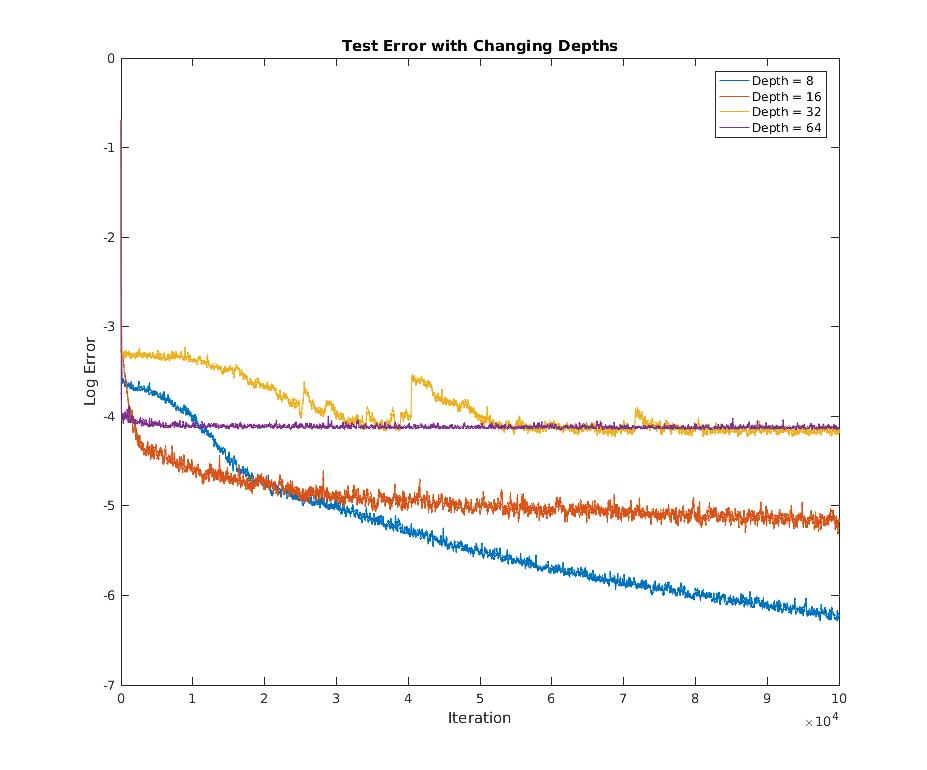
\includegraphics[width = 1.6in]{plotChangeDepth.jpg}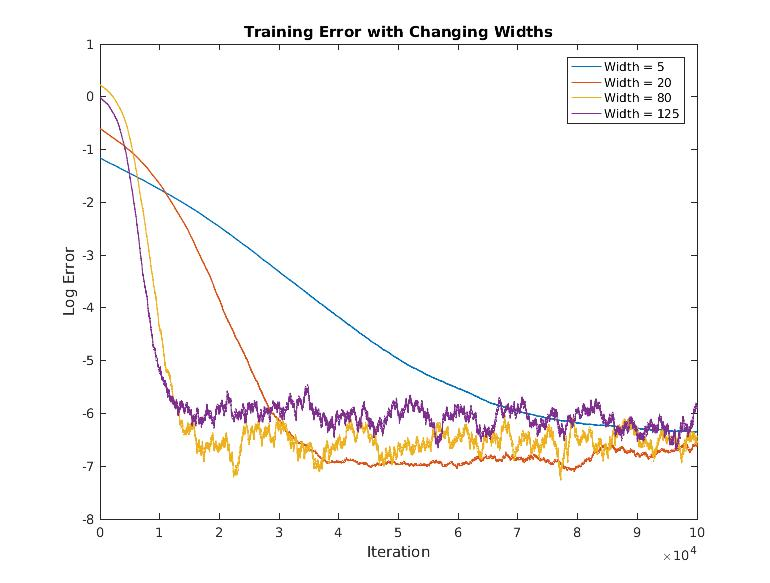
\includegraphics[width = 1.77in]{plotChangeWidth.jpg}
\caption{Left:Test Error of Networks of Varying Depth. Right: Test Error of Networks of Varying Width.}
\end{center}
\vskip -0.1in
\end{figure}
We note that we have been using training error as a measure of success, but it's possible that the true underlying parameters are not learned. If our loss function were strongly convex, small training error would imply a small norm in the parameter space. For the sign activation function, we can show a related result.

\begin{restatable}{theorem}{signUnique}
\label{SignUnique}
Let $\mathcal{M} = S^{d-1}$ and $\sigma$ be the sign activation function and $b_2,...,b_k = 0$. If the loss \eqref{errLoss} at $(\boldsymbol{a,\theta})$ is less than $O(1)$, then there must exist $\theta_i$ such that $w_1^T\theta_i > \Omega(1/\sqrt{k})$.
\end{restatable}



\section{Conclusion}

In this work, we view deep learning of neural networks in the context of electron-proton dynamics and analyzed the convergence of the underlying weight parameters of the neural network using arguments inspired from physics and non-convex optimization. To do so, we first established mathematical relationship between activation functions and their corresponding potentials. Next, we interpreted gradient descent as electrodynamics under a certain potential. Finally, we discovered classes of activation functions that give rise to positive convergence results, some of which relate to very commonplace activations, such as the sign and polynomial. For these classes of depth-2 neural networks, our results imply that they are provably learnable by deep learning. Our experiments seem to imply that higher depth neural networks are not learnable. 

However, we believe that convergence results for depth-2 neural networks can be extended to even more activation functions, such as the sigmoid or the ReLU. Also, we believe these convergence results can be proven with minimal assumptions. We hope that our work is a step in the theoretical understanding of the performance of neural networks seen in practice.




\bibliographystyle{icml2017}
\bibliography{biblio}

\newpage
\appendix


\section{Realizable Potentials}
\label{realizable}

\subsection{Activation-Potential Calculations}
First define the {\it dual} of a function $f: \R \to \R$ is defined to be 
%
\[ \widehat{f}(\rho) = E_{X,Y \sim N(\rho)}[f(X)f(Y)],\]
%
where $N(\rho)$ is the bivariate normal distribution with $X, Y$ unit variance and $\rho$ covariance. This is as in \cite{DanielyFS16}.
%
\begin{lemma}\label{rotLem}
Let $\mathcal{M} = S^{d-1}$ and $\sigma$ be our activation function, then $\widehat{\sigma}$ is the corresponding potential function.
\end{lemma}

\begin{proof}
If $u, v$ have norm 1 and if $X$ is a standard Gaussian in $\R^d$, then note that $X_1 = u^TX$ and $X_2 = v^TX$ are both standard Gaussian variables in $\R^1$ and the covariance is $E[X_1X_2] = u^Tv$. 

Therefore, the dual function of the activation gives us the potential function.
\begin{align*}
E_{X}[\sigma(u^TX)\sigma(v^TX)] & =
E_{X,Y \sim N(u^Tv)}[\sigma(X)\sigma(Y)] \\
& = \widehat{\sigma}(u^Tv).
\end{align*}
\end{proof}

By Lemma \ref{rotLem}, the calculations of the activation-potential
for the sign, ReLU, Hermite, exponential functions are given in
\cite{DanielyFS16}. For the Gaussian and Bessel activation functions,
we can calculate directly. In both case, we notice that we may write
the integral as a product of integrals in each dimension. Therefore,
it suffices to check the following 1-dimensional identities.
\begin{align*}
  & \int_{-\infty}^\infty
    \sqrt{2}e^{x^2/4}e^{-(x-\theta)^2}\sqrt{2}e^{x^2/4}e^{-(x-w)^2} \frac{1}{\sqrt{2\pi}} e^{-x^2/2}\, dx \\
  & \qquad = \sqrt{\frac{2}{\pi}}\int_{-\infty}^\infty
    e^{-(x-\theta)^2}e^{-(x-w)^2} \, dx = e^{-(\theta -w)^2/2}
\end{align*}
\begin{align*}
& \int_{-\infty}^\infty (\frac{2}{\pi})^{3/2}e^{x^2/2}K_0(|x-\theta|)K_0(|x-w|)  \frac{1}{\sqrt{2\pi}} e^{-x^2/2}\, dx \\
& \qquad 
= \int_{-\infty}^\infty \frac{2}{\pi^2}K_0(|x-\theta|)K_0(|x-w|) \, dx
  = e^{-|\theta -w|}
\end{align*}


The last equality follows by Fourier uniqueness and taking the Fourier transform of both sides, which are both equality $\sqrt{2/\pi}(\omega^2+1)^{-1}$. 



\subsection{Characterization Theorems}

\tranReal*

\begin{proof}
Let $h(x) = \mathfrak{F}^{-1}(\sqrt{\mathfrak{F}(f)})(x)$ and this is well-defined since the fourier transform was non-negative everywhere. Now, let $\sigma(x,w) = (2\pi)^{1/4}e^{x^2/4}h(x-w)$ and by assumption, it is bounded almost everywhere. Realizability follows by checking:
%
\begin{align*}
    E_{X \sim N}[\sigma(X,w)\sigma(X,\theta)]  &= \int_{\R^n} h(x-w)h(x-\theta) \, dx \\
    &= \int_{\R^n} h(x)h(x-(\theta-w)) \, dx \\
    &= \mathfrak{F}^{-1}(\mathfrak{F}(h\ast h)(\theta -w)) \\
    &= \mathfrak{F}^{-1}(\mathfrak{F}(h)^2(\theta - w)) \\
    &= \mathfrak{F}^{-1}(\mathfrak{F}(f)(\theta - w)) \\
    &= f(\theta - w) 
\end{align*}
\end{proof}




\rotReal*

\begin{proof}
By \ref{rotLem} and due to the orthogonality of hermite polynomials, if $f = \sum_i a_i h_i$, where $h_i(x)$ is the i-th Hermite polynomial, then
%
\[\widehat{f}(\rho) = \sum_{i} a_i^2 \rho^i\]

Therefore, any function with non-negative taylor coefficients is a valid potential function, with the corresponding activation function determined by the sum of hermite polynomials, and the sum is bounded almost everywhere by assumption.
\end{proof}

\section{Extra Stuff in section 3}
\todo{Clean this up later}






\begin{conjecture}
 Let $\mathcal{M} = S^{d-1}$ and $L$ be as in \eqref{errLoss} and $\sigma$ is the sign activation function. Then, almost surely over random choices of $b_1,...,b_k$, all critical points $(\boldsymbol{a,\theta})$ of $L$ with $a \neq 0$ are not local minima, except at the global minima. 
\end{conjecture}



\section{Generalization Error and Iteration Bounds}
\label{finite}
 
The design and analysis of gradient descent has so far assumed that we can calculate expectations perfectly. In reality, these expectations are instead replaced with empirical means. The approximate calculation of our potential and all its derivatives with samples are justified by the generalization error bounds implied by Rademacher complexities. 

Unfortunately, we cannot directly use the Gaussian distribution as it is unbounded. Therefore, we assume that our drawing distribution is the truncated Gaussian distribution in $\R^d$ such that our samples are always bounded in $l_2$ norm by $B$. We will show that applying this truncation will not affect the expectation very much. 

\begin{definition}
$Y$ follows a truncated Gaussian distribution at $B$ in $\R^d$ if $Y = X | ( \|X\| \leq B)$, where $X$ is a standard Gaussian in $\R^d$ and $ X \Big|S$ indicates the random variable $X$ conditioned on event $S$.
\end{definition}
%
\begin{lemma}
\label{choppedLem}
Let $f : \R^d \to \R$ be a function such that $|f(x)| \leq c\|x\|^p$. Let $X$ be a standard Gaussian in $\R^d$ and let $Y$ be a truncated Gaussian at $B$. Then, there exists $B = poly(d,p,\log(1/\epsilon))$ such that 
\[ \left|\expt[f(X)] - \expt[f(Y)] \right| \leq \epsilon\]
\end{lemma}

\begin{proof}
By standard concentration bounds and analysis, 
\begin{align*}
& |E[f(X)] - E[f(X)| \|X\|\leq B]| \\
& \qquad \leq (\frac{1}{P(\|X\|\leq B)}- 1) E[|f(X)|{\bf 1}_{\|X\|\leq B}]| \\
& \qquad \qquad + |E[f(X){\bf 1}_{\|X\|>B}]| \\
& \qquad \leq E[|f(X)|{\bf 1}_{\|X\|>B}] + 2cB^pe^{-B^2/8d}
\end{align*}


Taking $B = poly(d,p,\log(1/\epsilon))$ will make the second term $< \epsilon/2$, then the first term is also bounded by:
\begin{align*}
  E[|f(X)|{\bf 1}_{\|X\|>B}] &\leq (2\pi)^d \int_B^\infty cr^pe^{-r^2/2}r^{d-1}\,dr \\
                             &\leq C(2\pi)^dB^{p+d}e^{-B^2/2} < \epsilon/2
\end{align*}
\end{proof}

Next, we can appeal to the following well-cited theorems and standard techniques. For a better understanding of the notation and theorems used, we refer the refer to \cite{bartlett2002rademacher}.
%
\begin{theorem}[\cite{bartlett2002rademacher}]
Consider a function class $\mathcal{F}$ of functions $f : \mathcal{X} \to [0,1]$. And let $ x_1,...,x_n \in \mathcal{X}$ be i.i.d. samples selected according to some distribution $\mathcal{D}$. Let the Rademacher complexity of $\mathcal{F}$ to be 
\[R_n (\mathcal{F}) = E_{x_i,\sigma_i}\left[\sup_{f \in \mathcal{F}} \left|\frac{2}{n}\sum_{i=1}^nf(x_i)\sigma_i\right|\right]\]

where $\sigma_i$ are Rademacher variables. Then, for any $n$ and $\delta \in (0,1)$, with probability at least $1-\delta$, 
\[|E_{X}[f(X)]  - \frac{1}{n}\sum_{i=1}^n f(x_i)| \leq R_n(\mathcal{F}) + \sqrt{\frac{8\ln(2/\delta)}{n}} \]
for all $f \in\mathcal{F}$ simultaneously.
\end{theorem}

For all of our polynomial time bounds, whether we are calculating the potential or its derivatives, we are interested in bounding the Rademacher complexity of the class of functions of the form $\sigma_1(x^T\theta) \sigma_2(x^Tw)$, where $\sigma_1,\sigma_2$ are scalar functions.
%
\begin{theorem}
Let $\mathcal{X} = \{x \in \R^d, \|x\|_2\leq B\}$ and let $\sigma_1,\sigma_2 : \R \to [-C,C]$ be $L$-Lipschitz functions. Consider the following class of functions
%
\[\mathcal{F}_{\sigma_1,\sigma_2} = \{x\to\sigma_1(x^T\theta) \sigma_2(x^Tw) | x\in\mathcal{X}, \theta, w \in S^{d-1}\}.\]
Then, \[R_n(\mathcal{F}_{\sigma_1,\sigma_2}) \leq 48CLB\sqrt{\frac{2}{n}}\]
\end{theorem}
\begin{proof}
First, let's define a simpler function class: $\mathcal{G} = \{x\to x^T\theta  | x\in\mathcal{X}, \theta \in S^{d-1}\}$. By simple Rademacher bounds on the class of linear functions \cite{kakade2009complexity}, 
 %
 \[R_n(\mathcal{G}) \leq B\sqrt{\frac{2}{n}}\]
%
Since $\sigma_1,\sigma_2$ are L-lipschitz, we apply standard structural results in \cite{bartlett2002rademacher}
%
\[R_n(\sigma_i\circ \mathcal{G}) \leq 2LB\sqrt{\frac{2}{n}}\]
%
Let $s(x) = x^2$, then $s$ is $2C$-Lipschitz when $|x|\leq C$, so 
%
\[R_n(s\circ \sigma_i\circ\mathcal{G}) \leq 8CLB\sqrt{\frac{2}{n}},
R_n(s\circ(\sigma_1\circ \mathcal{G} +\sigma_2\circ \mathcal{G})) \leq
32 CLB\sqrt{\frac{2}{n}}\]
 
Since $2\sigma_1(x^T\theta)\sigma_2(x^Tw) = (\sigma_1(x^T\theta)+\sigma_2(x^Tw))^2 - \sigma_1(x^T\theta)^2 - \sigma_2(x^Tw)^2$, we conclude that 
\[R_n (\mathcal{F}_{\sigma_1,\sigma_2}) \leq 48CLB\sqrt{\frac{2}{n}}\]
\end{proof}

\begin{theorem}
\label{genErrBound}
Let $\mathcal{M} = S^{d-1}$ and $L$ be as in \ref{errLoss} with potential function $\Phi$ corresponding to activation $\sigma$. Assume that $|\sigma(x)|, |\sigma'(x)|,|\sigma''(x)|, |\sigma'''(x)|$ are all $O(|x|^p)$ for some $p$.  

Then, in $poly(d^p,1/\epsilon, \log(1/\zeta))$ samples, we can compute $\hat{L}$ such that with probability $1-\zeta$, we have simultaneously $\|\widehat{L}(x) -L(x)\|, \|\nabla \widehat{L}(x) = L(x)\|, \|\nabla^2\widehat{L}(x) -\nabla^2 L(x)\| \leq \epsilon$ for all $x\in \Omega$.
\end{theorem}

\begin{proof}
  We first bound the generalization error of each $\Phi$. Notice that
  our approximation to $\Phi$ is done by first drawing $n$
  i.i.d. samples $x_i \sim \mathcal{D}_B$, where $\mathcal{D}_B$ is
  the Gaussian in $\R^d$ truncated by the ball of radius
  $B = poly(d,p,\log(1/\epsilon))$. Then, we calculate the empirical
  average.
%
\[\widehat{\Phi}(\theta,w) = \frac{1}{n}\sum_{i=1}^n \sigma(x_i^T\theta)\sigma(x_i^Tw) \]

Since $|x_i^T\theta|\leq B$, we conclude that $\sigma, \sigma'$ is bounded by $poly(B^p)$. Therefore, by our error bound theorems and by simple union bounds over the $poly(k) = poly(d)$ sum of $\Phi$, we conclude that with probability $1-\zeta$, if we choose $n = poly(d^p,1/\epsilon, \log(1/\zeta))$, we have 
%
\[|E_{X\sim \mathcal{D}_B}[\sigma(X^Tw)\sigma(X^T\theta)] -
\widehat{\Phi}(\theta^Tw)| \leq \epsilon/2,\]
for all $\theta, w \in \mathcal{M}$. And combining with Lemma
\ref{choppedLem}, we conclude that
$|\widehat{\Phi}(\theta,w) - \Phi(\theta,w)|\leq \epsilon$. We proceed
with the same proof for the first and second derivatives and use a
union bound to derive our claim.
\end{proof}

\subsection{Infinite Iteration Bounds} 
\label{InfIter}


\begin{theorem}\cite{lee2016gradient, PanageasP16}\label{convStrict}
  Let $f :\Omega \to \R$ be a twice differentiable function such that
  $\sup_{x \in \Omega} \|\nabla^2 f\| \leq L$. Let
  $\mathcal{S} \subseteq \Omega$ be the set of critical points of $f$
  that are not local minima. Also, if
  $g(x) = x - \frac{1}{2L} \nabla f(x)$, then
  $g(\Omega) \subseteq \Omega$.

  Then, running Algorithm \ref{GD} with gradient input $\nabla f$ and
  stepsize $\alpha = 1/(2L)$, as the iteration $T \to\infty$, will
  converge to a point $x_\infty$ outside of $S$ almost surely over
  randomly chosen initial points $x_0$.
\end{theorem}

\begin{corollary}
Assume all the assumptions of Theorem \ref{convStrict} and let $f$ admit a global minima in $\overline{\Omega}$. Assume all critical points of $f$ in $\Omega$ are not local minima, except at the global minima. Then, running Algorithm \ref{GD} with gradient input $\nabla f$ and stepsize $\alpha = 1/(2L)$ will converge to the global minima almost surely as the iteration count $T \to\infty$.
\end{corollary}

\subsection{Finite Iteration Bounds} 
To derive a finite iteration bound, we will apply stochastic gradient descent to our objective function and use standard martingale techniques for analysis. We will need to slightly alter the main result in \cite{GeHJY15} because we lack strong convexity assumptions. Also, we will accordingly alter the stochastic gradient descent algorithm to terminate upon finding a critical point that is $\gamma$-strict, for small $\gamma$.
%
\begin{algorithm}[hb]
 \caption{$x = SGD(\widehat{L}, x_0, T,\alpha,\epsilon)$}
   \label{SGD}
\begin{algorithmic}
   \STATE {\bfseries Input:} $\widehat{L}:\mathcal{M} \to \R$; $x_0 \in \mathcal{M}$; $T\in \N$; $\alpha \in \R$; $\epsilon\in\R$
   \vspace{.1in}
   \STATE {\bf Initialize} $x = x_0$
   \FOR{$i=1$ {\bfseries to} $T$}
   \STATE Sample $\eta$ uniformly on unit sphere.
   \STATE $x = x - \alpha(\nabla \widehat{L} (x)+\eta)$ 
   \STATE $x = \Pi_\mathcal{M} x$
   \IF{$\|\nabla\widehat{L}(x)\|\leq 2\epsilon/3$ {\bf and} $\lambda_{min}(\nabla^2\widehat{L}(x)) \geq -2\epsilon/3$}
   \STATE {\bf return} $x$
   \ENDIF
   \ENDFOR
   \STATE {\bf return} FAIL
\end{algorithmic}
\end{algorithm}





\begin{theorem}\label{strongConverge}
Let $L :\Omega \to \R$ be a twice differentiable function such that $|L(x)| \leq B, \|\nabla^2 L(x)\| \leq C,\|\nabla^2L(x) -\nabla^2L(y)\| \leq \rho\|x - y\|$ for all $x,y\in\Omega$. Also, assume that we access to stochastic function $\widehat{L}$ such that $\|\widehat{L}(x) -L(x)\|, \|\nabla \widehat{L}(x) = L(x)\|, \|\nabla^2\widehat{L}(x) -\nabla^2 L(x)\| \leq \epsilon/3$ for all $x\in \Omega$.

Then, we can choose stepsize $\eta = 1/poly(d,B,C,\rho,1/\epsilon,\log(1/\zeta))$, such that with probability at least $1-\zeta$, running Algorithm \ref{SGD} on $\widehat{L}$ with stepsize $\eta$  returns a point that is in $\mathcal{M}_\epsilon$ after at most $poly(d,B,C,\rho,1/\epsilon, \log(1/\zeta))$ iterations.
\end{theorem}

\begin{proof}
If Algorithm \ref{SGD} succeeds, then by triangle inequality and our error bounds on the stochastic function $\widehat{L}$ and its derivatives, we know that $x \in \mathcal{M}_\epsilon$. So, it suffices to argue that our algorithm succeeds with high probability.

By \cite{GeHJY15} Lemma 7 and 9, we see that if
$x_i \not \in\mathcal{M}_{\epsilon/3}$ for all the iterations, then in
expectation, our objective function decreases by $poly(\eta)$ and by
using Azuma's inequality, this occurs with probability
$1-\zeta$. Since our objective function is bounded by $poly(d,B)$, we
conclude that stochastic gradient descent must have encountered a
point $x_i$ such that $x_i \in \mathcal{M}_{\epsilon/3}$ after at most
$poly(d,B,C,\rho,1/\epsilon,1/\gamma, \log(1/\zeta))$. Then, by our
bounds on $\widehat{L}$ and $L$, we conclude that both
$\|\nabla\widehat{L}(x_i)\| \leq 2\epsilon/3$ and
$\lambda_{min}(\nabla^2 \widehat{L}(x_i)) \geq -2\epsilon/3$. So, our
algorithm succeeds with probability $1-\zeta$.
\end{proof}



\section{Convergence of Almost Strictly Subharmonic Potentials}\label{App:Subharm}

For concreteness, we will focus on a specific potential function with this property: the Gaussian kernel $\Phi(\theta, w) = \exp(-\|\theta - w\|^2/2)$. In $\R^d$, the Laplacian is $\Delta \Phi = ( \|\theta - w\|^2 -d ) \exp(-\|\theta - w\|^2/2)$, which becomes positive when $\|\theta - w \|^2 \geq d$. Thus, $\Phi$ is strictly subharmonic outside a ball of radius $\sqrt{d}$. This informally implies that $\theta_1$ converges to a $\sqrt{d}$-ball around some $w_j$. 

When $a$ is fixed under Assumption \ref{outputFixed}, the node-wise
SGD algorithm is given by Algorithm \ref{GDNode}. For the Gaussian, we
are only able to derive exponential time bounds on the runtime due to
the fast decay of the potentials. Note that Gaussian potential
restricted to $S^{d-1}$ gives rise to the exponential activation
function, so we can show convergence similarly.

\begin{algorithm}[hb]
 \caption{Node-wise SGD Algorithm}
   \label{GDNode}
\begin{algorithmic}
   \STATE {\bfseries Input:} $\theta = (\theta_1,...,\theta_k), \theta_i \in \mathcal{M}$; $T\in \N$; $\widehat{L}$; $\alpha\in \R$; $\delta \in \R$
   \vspace{0.1in}
   \STATE {\bf Initialize} $a = 0$
   \FOR{$i=1$ {\bfseries to} $k$}
   \STATE $a_i = -1$
   \STATE  $\theta_i =  SGD( \widehat{L}_{\theta_i},\theta_i,T, \alpha,\delta)$
   \ENDFOR
   \STATE {\bf return} $\theta = (\theta_1,...,\theta_k)$
\end{algorithmic}
\end{algorithm}
%\gaussStrict*

\begin{restatable}{theorem}{gaussStrict}
\label{GaussStrict}
Let $\mathcal{M} = \R^d$ and $\Phi(\theta,w) = e^{-\|a-b\|^2/2}$ and Assumption \ref{outputFixed} holds. If $2d < \|\theta_i - w_j\|^2 < O(d)$ for all $i, j$, then $\theta = (\theta_1,...,\theta_k)$ is a $e^{-O(d)}$-strict point of our simplified loss \eqref{errFixed}.

Let $w_1,...,w_k$ are randomly initialized according to $\mathcal{N}(0, c*{\bf I}_{d\times d})$, for some constant $c > 2$ such that $kc^2e^{-c} \leq e^{-2d}$. Then, with high probability, running Algorithm \ref{GDNode} initialized with $\theta = 0$, and error  $\delta = e^{-O(d)}$, and stepsize $\alpha = e^{-O(d)}$ returns a point $\theta$ that is within $e^{-O(d)}$ of the global minima in $T = e^{O(d)}$ number of iterations.
\end{restatable}

\begin{proof}
Consider again a correlated movement, where each $\theta_i$ are moved along the same direction $v$. As before, this drops the pairwise $\theta_i$ terms, so since $O(d) > \|\theta_i -w_j\|^2 > 2d$, we see that $\Delta_{\theta_i} \Phi = (\|\theta_i -w_j\|^2 - d)\Phi(\theta_i,w_j) > e^{-O(d)}$. 
%
\[\Tr(\nabla^2 L) = -2\sum_{i=1}^k \sum_{j=1}^k \Delta_{\theta_i}\Phi(\theta_i, w_j) < -e^{-O(d)}\]

Therefore, $\nabla^2 L$ must admit a strictly negative eigenvalue that
is less than $e^{-c_3 d}$, which implies our claim (we drop the
$poly(d,k)$ terms).

Now, we proceed with the convergence proof. Consider the gradient descent output of the first node $\theta_1$. The loss function is given by:
%
\[L(\theta_1) =  - 2\sum_{j=1}^k \Phi(\theta_1,w_j)\]

By standard Chernoff bounds, we have $\|w_i\|^2 < 3cd$ for all $i$ and $\|w_i -w_j\|^2 \in (1.5cd, 2.5cd)$ for all $i, j$ with high probability as $k = poly(d)$. We just need to consider $\Omega = \{ x \in \R^d | \|x \|^2 < 3cd\}$ since the convex hull of $w_i$ is contained in $\Omega$ and so the gradient operator $g$ satisfy $g(\Omega) \subseteq \Omega$ (the gradient outside the convex hull points towards the convex hull).  

To use Thm \ref{strongConverge}, we check the regularity conditions: note that we can choose $L, B, \rho$ to be $poly(d)$ since the first, second and third partials of $\Phi$ are all bounded by $poly(d)$. Now, by choosing $\epsilon = e^{-O(d)}$ for some $c$, we know that with high probability, running SGD in $T = e^{O(d)}$ iterations will output $\theta_1$ such that 1) $\|\nabla L (\theta_1)\| < e^{-O(d)}$ and 2) $\lambda_{min}(\nabla^2L(\theta_1)) > -e^{-O(d)}$.

WLOG, $w_1$ be a closest point to $\theta_1$. Since  $\lambda_{min}(\nabla^2L(\theta_1)) > -e^{-O(d)}$, by the first part of our claim, $\|w_1 - \theta_1\|^2 < 1.1d$ and from triangle inequality, $\|w_i - \theta_1 \|^2 > c*d$ for all $i \neq 1$. 

Next, we calculate the gradient value at $\theta_1$, 
\begin{align*}
\|\nabla L(\theta_1)\| & = \|2\sum_{j=1}^k
                         \nabla_{\theta_1}\Phi(\theta_1,w_j)\| \\
& \geq \|\nabla_{\theta_1} \Phi(\theta_1,w_1) \| - \|\sum_{j>1}
  \nabla_{\theta_1}\Phi(\theta_1,w_j)\| \\
& \geq \|\theta_1-w_1\|e^{-1.1d} - kc^2e^{-cd} \geq e^{-O(d)} 
\end{align*}

Therefore, $\epsilon = e^{-O(d)}$ can be chosen small enough to ensure that $\|\theta_1 - w_1\| = e^{-O(d)}$. 

Finally, we proceed by induction. Since $\theta_1, w_1$ are paired to high accuracy, we note that we can treat it as if $w_1, \theta_1$ are removed from our loss equation. Therefore, we conclude that for all $\theta_i$, it will match with some $w_{\pi(i)}$ for some permutation $\pi$, with error $e^{-O(d)}$. 
\end{proof}




\section{Convergence of Almost $\lambda$-Harmonic Potentials}\label{App:EigenFunc}


When the output weights are variable, notice that our convergence results often rely on the optimality of the output weights. For this reason, we will optimize the output weights at every gradient descent step, by carefully choosing the stepsize. As our loss function \eqref{errLoss} is quadratic in $a$, we know that gradient descent will find $a^*$ efficiently. 
%
\begin{theorem}\cite{nesterov2013introductory}\label{quadConverge}
  Let $x_0 \in \Omega = \{ x \in \R^d | \|x \| \leq poly(d)\}$ and let
  $L(x) = x^TAx + b^Tx$ be a quadratic loss, where $A$ is a positive
  semi-definite matrix with maximum eigenvalue $\beta$. Then, running
  Algorithm \ref{GD} on $L$ with stepsize $\alpha = 1/\beta$ converges
  to $x_T$ such that
  \[L(x_T) - \min_{x \in \Omega} L(x) \leq \epsilon\]
  in $T = poly(d, \beta, 1/\epsilon)$ iterations.
\end{theorem} 

\noindent The pseudocode is given in Algorithm \ref{NodeGDOpt}. 
%
\begin{algorithm}[tb]
 \caption{Node-wise Gradient Descent Algorithm with Output Weights Optimization}
   \label{NodeGDOpt}
\begin{algorithmic}
  \STATE {\bfseries Input:}
  $(\boldsymbol{a,\theta}) = (a_1,...,a_k,\theta_1,...,\theta_k), a_i
  \in\R, \theta_i\in\mathcal{M}$;
  $T\in \N$; $\widehat{L}$; $\alpha\in \R$; $\delta \in \R$;
  $\gamma \in R$; \vspace{0.1in} \STATE{\bf Initialize} $a = 0$
  \FOR{$i=1$ {\bfseries to} $k$} 
  \REPEAT \STATE Sample $\theta_i$
  uniformly from $\mathcal{M}$
  \UNTIL{$\left (\frac{\partial
        \widehat{L}(\boldsymbol{a,\theta})}{\partial a_i} \right)^2
    \geq \gamma$}
  \FOR{$j=1$ {\bfseries to} $T$} \STATE
  $a_i = a_i^* = GradientDescent \left(\widehat{L}_{a_i}, a_i, 1,
    \frac{\partial^2 \hat{L}}{\partial a_i^2} \right)$
  \STATE
  $\theta_i = SGD \left(\widehat{L}_{\theta_i}, \theta_i,1, \alpha,\delta \right)$
   \ENDFOR
   \STATE    $a =  GradientDescent \left(\widehat{L}_{a_1,..,a_i},
     (a_1,..,a_i), T , \alpha \right)$\;
   \ENDFOR
   \STATE {\bf return} $a = (a_1,...,a_k), \theta = (\theta_1,..., \theta_k)$
   \end{algorithmic}
\end{algorithm}


First, we need some control on the size of the squares of variable charges, $a_i^2$. Node-wise gradient descent allows us to maintain that control. We will work with \eqref{errEmp} and let $\widehat{Phi}$ be the empirical potential function.

\begin{theorem}\label{nonDecrease}
  Let $\widehat{\Phi}(\theta, w)$ be $poly(d)$-Lipschitz in $\theta$,
  $|\widehat{\Phi}| \leq poly(d)$ on $\mathcal{M}$, and $\sum_{j \neq i} |a_j| + \sum_j |b_j| \leq poly(d)$. Also, assume that if $\theta_i$ is drawn uniformly on $\mathcal{M}$,
%
\[\expt_{\theta_i}\left[\left(  \sum_{j\neq i} a_j \widehat{\Phi}(\theta_i,\theta_j) + \sum_{j=1}^k b_j \widehat{\Phi}(\theta_i,w_j)\right)^2\right] \geq \epsilon \]
%
Then, with high probability, running Algorithm \ref{NodeGDOpt} on $\widehat{L}$ with stepsize at most $\alpha = 1/poly(d)$ and $\gamma = \epsilon$ will enforce that $a_i^2 = \Omega(\epsilon)$ when running SGD on $\theta_i$. The sample complexity is $poly(d,1/\epsilon)$
\end{theorem}

\begin{proof}
We want to show that $a_i^2 = \Omega(\epsilon)$. First, we analyze the random drawing of $\theta_i$.  Let 
%
\[  \widehat{C}(\theta_i) = \sum_{j\neq i} a_j \widehat{\Phi}(\theta_i,\theta_j) + \sum_{j=1}^k b_j \widehat{\Phi}(\theta_i,w_j)\]
%

By assumption, we know that $\expt[\widehat{C}(\theta_i)^2] \geq
\epsilon$. Since $a_i,b_i, \widehat{\Phi}$ is $poly(d)$-bounded, then $\widehat{C}(\theta_i)$ is $poly(d)$-bounded. From Hoeffding bounds, we see that after $poly(d,1/\epsilon)$ samples, we know that $\hat{\expt}\widehat{C}(\theta_i)^2 \geq \epsilon/2$, where $\hat{\expt}$ denotes the empirical average over $\theta_i$. Therefore, we must have found some $\theta_i$ such that $\widehat{C}(\theta_i)^2 \geq \epsilon/2$. \Snote{I don��t think Hoeffding��s bounds apply here. If Phi is always bounded, you can just apply a Markov argument here}.\Rnote{Direct Markov goes the wrong direction. Hoeffding applies to bounded variables so I believe this works?}


Next, notice that $\hat{L}$ is a quadratic in $a_i$, which is a
scalar. Therefore, the gradient step on $a_i$ is chosen with the exact
stepsize that will optimize $a_i = a_i^*(\theta_i)$.  By optimality of
$a^*$,
%
\begin{equation}
0 = 2a_i \widehat{\Phi}(\theta_i,\theta_i) + 2\sum_{j\neq i} a_j \widehat{\Phi}(\theta_i,\theta_j) + 2\sum_{j=1}^k b_j \widehat{\Phi}(\theta_i,w_j)
\end{equation} 
%
Therefore, 
%
\begin{align*}
 a_i^* & = - \frac{1}{\widehat{\Phi}(\theta_i,\theta_i)} (\sum_{j\neq i} a_j \widehat{\Phi}(\theta_i,\theta_j) + \sum_{j=1}^k b_j \widehat{\Phi}(\theta_i,w_j)) \\
& = -\frac{1}{\widehat{\Phi}(\theta_i,\theta_i)}\widehat{C}(\theta_i) 
\end{align*}

\Snote{ Is $\widehat{\Phi}$ computable efficiently? What about $\widehat{C}$?}


As $a_i$ is initially $0$ when sampling $\theta_i$, we conclude that we can find $\theta_i$ such that
%
\[ \left( \pd{\hat{L}}{a_i} \right)^2 = 4 \widehat{C}(\theta_i)^2 \geq \epsilon.\]
Therefore, after $poly(d,1/\epsilon)$ samples, our sampling algorithm will, with high probability, return $\theta_i$  such that $a_i^2 = a_i^*(\theta_i)^2 \geq \epsilon /4$. 
\Snote{ Is computable efficiently? What about $\widehat{C}$?}
\Rnote{Depends on how many samples you choose. It is true that the sample complexity of this algorithm  going to be superpolynomial for $\lambda$-harmonic. Iteration complexity is poly. For the polynomial activation, everything is poly}
Next, we examine the SGD steps. Note
%
\begin{align*}
\nabla_{\theta_i} \widehat{C}(\theta_i) & =  \sum_{j\neq i} a_j \nabla_{\theta_i}\widehat{\Phi}(\theta_i,\theta_j) + \sum_{j=1}^k b_j \nabla_{\theta_i}\widehat{\Phi}(\theta_i,w_j) \\
& = \frac{1}{2a_i^*} \nabla_{\theta_i}\widehat{L}
\end{align*}

Now, we calculate the following gradient: 
%
\begin{equation}
\nabla_{\theta_i} (a_i^*)^2 = 2a_i^*\frac{-1}{\widehat{\Phi}(\theta_i,\theta_i)} \nabla_{\theta_i} \widehat{C}(\theta_i) = \frac{1}{\widehat{\Phi}(\theta_i,\theta_i)} (-\nabla_{\theta_i} \widehat{L})
\end{equation}

Therefore, let $\theta_{i}^{(j)}$ be the value of $\theta_i$ in the $j$-th iteration of SGD with stepsize $\alpha$. Since $\theta_i$ moves in the direction of the gradient of $(a_i^*)^2$ in expectation and $(a_i^*)^2$ is $poly(d)$-Lipschitz in $\theta_i$, so we conclude by a standard analysis of SGD with stepsize $\alpha = 1/poly(d)$ that $(a_i^*)^2$ is a supermartingale with a bounded difference of $1/poly(d)$. Specifically, let $\widetilde{\nabla}_{\theta_i}\hat{L}$ be the stochastic gradient with $E[\widetilde{\nabla}_{\theta_i}\hat{L}] = \nabla_{\theta_i}\hat{L}$.
%
\[E[a_i^*(\theta_i^{(j+1)})^2 | \theta_{i}^{(j)}] = E[a_i^*(\theta_i^{(j)} - \alpha \widetilde{\nabla}_{\theta_i} \hat{L})^2 |\theta_{i}^{(j)}] \]
\[\geq a_i^*(\theta_i^{(j)})^2 - \alpha E[(\nabla_{\theta_i}(a_i^*)^2)^T\widetilde{\nabla}_{\theta_i}\hat{L}]\]
%
\[+ poly(d)\alpha^2E[\|\widetilde{\nabla}_{\theta_i}\hat{L} - \nabla_{\theta_i}\hat{L}\|^2 - \|\nabla_{\theta_i}\hat{L}\|^2]\]
%
\[\geq a_i^*(\theta_i^{(j)})^2 + \alpha \|\nabla_{\theta_i}\hat{L}\|^2 - (\alpha/2) \|\nabla_{\theta_i}\hat{L}\|^2 \geq a_i^*(\theta_i^{(j)})^2  \]

Therefore, $X_j = a_i^*(\theta_i^{(j)})^2$ is a supermartingale and by Azuma's, that in $poly(1/\epsilon,d,\log(1/\zeta))$ iterations, $(a_i^*)^2 = \Omega(\epsilon)$ with probability $1-\zeta$. By choosing $\zeta$ to be exponentially small, we may union bound over the $poly(d,1/\epsilon)$ iterations of SGD to derive our conclusion.
\end{proof}

\begin{definition}
$\Phi(\theta, w)$ is $(\lambda,m)$-Harmonic on $S^{d-1}$ if for all $\theta, w\in \Omega$, $|\Delta_{\theta}\Phi(\theta, w) - \lambda \Phi (\theta,w)| \leq |\theta^Tw|^m$ 
\end{definition}
\Rnote{Not sure if there is a nice general definition to be honest...to be discussed}


\eigConv*
%
\begin{proof}
We start with the construction. Let $u,v$ be on the unit sphere, and WLOG let $v = (0,...,1)$. Then, we can reparametrize any function of the dot product $f(u^Tv) = f(\cos(\theta))$, where $\theta \in [0, \pi]$ is the angle between $u$ and the positive $z$-axis.
Using the Laplacian formula on $S^{d-1}$ gives:
\begin{align*}
\Delta f & = (\sin \theta)^{2-d} \frac{\partial}{\partial \theta}\left[ (\sin \theta)^{d-2} \frac{\partial f(\cos \theta)}{\partial \theta}\right] \\
& = f''(\cos\theta)(\sin \theta)^{2} - (d-1)\cos(\theta)f'(\cos\theta)
\end{align*}

We want $f$ to be approximately $1$-harmonic, so we want to approximately solve:
%
\[f''(x)(1-x^2) - (d-1)xf'(x) =  f(x) \]

Let us construct our approximate function $f$ as follows. Let $c_n$ are the Taylor coefficients of $f(x)$, then we want to solve the equation:
Therefore, we get the following recurrence: $c_n (n(n-1) + (d-1)*n + 1) = c_{n+2} (n+2)(n+1)$. Let $c_0 = 1, c_1 = 0$, then we run this recurrence holds $n=0,...,N-2$ for some $N$ even and set $c_{N+i} = 0$ for $i > 0$, then
\begin{align*}
\Delta f & = f''(\cos\theta)(\sin \theta)^{2} - (d-1)\cos(\theta)f'(\cos\theta) \\
&= f(\cos(x)) + k_N(\cos\theta)^N
\end{align*}

Where $k_N = N^2 + (d-2)N + 1$. Notice that $f(x)$ has non-negative Taylor coefficients and is a bounded polynomial, so $f$ is a realizable potential function by Theorem \ref{thm:rotReal}. We can also choose $N$ to be odd by setting $c_0 = 0, c_1 = 1$. Therefore, we can construct a realizable $(1, m)$-Harmonic potential for any $m$.

We show our result under this potential function $\Phi = f$ and then we can normalize later. We first show a weaker result: each $(a_i,\theta_i)$ must satisfy (i) there exists $j$ such that $|w_j^T\theta_i| > 1-\epsilon$, or (ii) $|a_i| < \epsilon$, or (iv) there exists $j\neq i$ such that $|\theta_j^T\theta_i| > 1-\epsilon$. Assume that $(\boldsymbol{a,\theta}) \in \mathcal{M}_{\epsilon^2/(4d)}$ and we have a $(a_i,\theta_i)$ that does not satisfy (i), (ii), (iv). Then,
%
\[|\pd{L}{a_i}| = |2\sum_{j=1}^k  b_j  \Phi(\theta_i^T w_j) +  2\sum_{j\neq i} a_j \Phi(\theta_i^T\theta_j)  + 2a_i\Phi(1)| \leq \epsilon \] 

And, 
%
\[\Delta_{\theta_i} L =  2\sum_{j=1}^k a_i b_j  (-\Phi(\theta_i^T w_j) \]
\[+ k_N(\theta_i^Tw_j)^N) +  2\sum_{j\neq i} a_i a_j(-\Phi(\theta_i^T\theta_j) + k_N(\theta_i^T\theta_j)^N)\]

Therefore,
%
\[|\Delta_{\theta_i}L + 2a_i^2\Phi(1)| \leq \epsilon |a_i| \]
\[+  2|a_i| k_N|\sum_{j=1}^k b_j (\theta_i^Tw_j)^N +  \sum_{j\neq i}  a_j(\theta_i^T\theta_j)^N|\]

Since (i), (iv) does not hold and $\|a\| \leq poly(d)$, we can choose $N = O(\frac{1}{\epsilon}\log(d))$ large enough such that 
%
\[ 2k_N |\sum_{j=1}^k b_j (\theta_i^Tw_j)^N +  \sum_{j\neq i}  a_j(\theta_i^T\theta_j)^N| \leq  2poly(d,k,N)e^{-\epsilon N} \]
\[\leq \epsilon/2\] 

Therefore, by (ii) and $\Phi(1) > 1$,
%
\[\Delta_{\theta_i} L \leq -2a_i^2 \Phi(1) +\epsilon |a_i|+(\epsilon/2)|a_i| \leq |a_i|(-2\epsilon \Phi(1) + 3\epsilon/2) \]
\[\leq -\epsilon^2/4\]

This implies that $(\boldsymbol{a,\theta})$ is $\epsilon^2/(4d)$-strict, contradicting that it is in $\mathcal{M}_{\epsilon^2/(4d)}$. 

Now, consider all $\theta_i$ such that only condition (iv) holds. WLOG, assume that these are $\theta_1,...,\theta_l$, for some $l \leq k$. Furthermore, assume that $|\theta_i^T\theta_j| \leq 1-\epsilon$ for $i \leq l, j\geq l+1$. Then, consider a correlated rotation on the sphere, which is a correlated translation in spherical coordinates $\widetilde{\theta_1},...,\widetilde{\theta_l}$. Now, consider the loss function

\[ H({\bf a, v}) = L({\bf a,\theta_1+v,...,\theta_l+v},\theta_{l+1},..\theta_k)\]

Therefore, Assume that $(\boldsymbol{a,\theta}) \in \mathcal{M}_{\epsilon^2/(4d)}$ and we have a $(a_i,\theta_i)$ that does not satisfy (i), (ii), (iii). Then, the optimality conditions on ${\bf a}$ are unchanged, we must have
%
\[\Delta_{{\bf v}} H =  2\sum_{i=1}^l\sum_{j=1}^k a_i b_j  (-\Phi(\theta_i^T w_j) \]
\[+ k_N(\theta_i^Tw_j)^N) +  2\sum_{i=1}^l\sum_{j= l+1}^k a_i a_j(-\Phi(\theta_i^T\theta_j) + k_N(\theta_i^T\theta_j)^N)\]

Therefore, from our optimality conditions
%
\[|\Delta_{{\bf v}}H + \sum_{i=1}^l 2a_i^2\Phi(\theta_i^T\theta_i) + 2\sum_{i \neq j}^l a_ia_j\Phi(\theta_i^T\theta_j)| \leq \epsilon |a_i| \]
\[+  2|a_i| k_N\sum_{i=1}^l|\sum_{j=1}^k b_j (\theta_i^Tw_j)^N +  \sum_{j=l+1}^k  a_j(\theta_i^T\theta_j)^N|\]

Again, since these inner products are assumed to be less than $1-\epsilon$, we can choose $N = O(\frac{1}{\epsilon}\log(d))$ large enough such that 
%
\[ 2|a_i| k_N\sum_{i=1}^l|\sum_{j=1}^k b_j (\theta_i^Tw_j)^N +  \sum_{j=l+1}^k  a_j(\theta_i^T\theta_j)^N|\]

\[ \leq  2poly(d,k,N)e^{-\epsilon N} \leq \epsilon/2\] 

Finally, we can rewrite that inequality in (iii) as 
%
\[D = \expt\left[\left( \sum_{i=1}^l a_i \sigma(\theta_i,X)\right)^2\right] \]
%
\[=\sum_{i=1}^l a_i^2\Phi(\theta_i^T\theta_i) + \sum_{i \neq j}^l a_ia_j\Phi(\theta_i^T\theta_j)\]
%
So, if (iii) does not hold, $D > \epsilon^2$ and combined with the fact that (ii) does not hold,
%
\[\Delta_{\theta_i} L \leq -2D +\epsilon |a_i|+(\epsilon/2)|a_i| \]

\[\leq -2\epsilon^2 + |a_i|(-2\epsilon \Phi(1) + 3\epsilon/2) \leq -\epsilon^2/4\]

This implies that $(\boldsymbol{a,\theta})$ is $\epsilon^2/(4d)$-strict, contradicting that it is in $\mathcal{M}_{\epsilon^2/(4d)}$. \\

Finally, there exists $\theta_{j_1},...\theta_{j_l}$ such that $|\theta_i^T\theta_{j_1}| > 1-\epsilon$ and $|\theta_{j_{i}}^T\theta_{j_{i+1}}| > 1-\epsilon$, and $|\theta_{j_l}^Tw_j| > 1-\epsilon$ for some $w_j$. Therefore, $|\theta_i^Tw_j| > 1- (l+1)\sqrt{\epsilon}$. By choosing $\epsilon' = \epsilon/poly(d)$, we get our claim. 
\end{proof}


\begin{theorem}
For any $\epsilon < 1/poly(d)$, we can construct a realizable potential $\Phi$ such that with high probability, running Algorithm \ref{NodeGDOpt} on \eqref{errLoss} with error $\delta = poly(\epsilon,1/d)$, $\gamma = \epsilon$ and stepsize $\alpha = 1/poly(d,1/\epsilon)$ converges in $T = poly(d, 1/\epsilon)$ iterations to $(\boldsymbol{a,\theta})$ such that either  $\theta$ is within $\epsilon$-neighborhood of the global minima or there exists $i$ such that if $\theta_i$ is picked uniformly in $\mathcal{M}$
%
\[ \expt\left[\left( \sum_{j < i} a_j \Phi(\theta_i,\theta_j) + \sum_{j=1}^k b_j \Phi(\theta_i,w_j)\right)^2\right] < \epsilon\]

The sample complexity is $d^{O(\log(d)/\epsilon)}$.
\end{theorem}

\begin{proof}
Let $\Phi_m$ be the $(1,m)$-Harmonic potential in Theorem \ref{eigConv} with $m = poly(d,1/\epsilon)$ and $m$ odd. We first consider the algorithm on node $\theta_1$ and claim that it will merge with some $w_j$ and then we will proceed with induction. 


If
%
\[ \expt\left[\left( \sum_{j < 1} a_j \Phi(\theta_i,\theta_j) +
    \sum_{j=1}^k b_j \Phi(\theta_i,w_j)\right)^2\right] < \epsilon,\]
then we are done. Otherwise, with high probability, Theorem
\ref{nonDecrease} allows us to deduce that throughout the SGD
algorithm applied on $\theta_1$, $a_1^2 = \Omega(\epsilon)$.

Now we want to apply Theorem \ref{strongConverge}, so we check the regularity conditions. Since $\mathcal{M} = S^{d-1}$, then we can choose $B, L, \rho$ to be $poly(d)$ since $\Phi$ and the second and third partials of $\Phi$ are all bounded by $poly(d)$. Furthermore, by our construction, our activation function $\sigma(x)$ and its derivatives are $O(|x|^{poly(d,1/\epsilon)})$. By Theorem \ref{genErrBound}, with high probability, we can construct a stochastic oracle up to $poly(\epsilon,1/d)$ error with sample complexity $d^{poly(d,1/\epsilon)}$.


Therefore, by Theorem \ref{strongConverge} we conclude that we converge to $\theta_1 \in \mathcal{M}_{poly(\epsilon,1/d)}$. By Theorem \ref{eigConv}, since $|a_i| = \Omega(\sqrt{\epsilon})$, this implies that it is in an $poly(\epsilon,1/d)$-neighborhood of some $w_{i}$ in $poly(d,1/\epsilon)$ time. Note that $\theta_1$ will close to with $\pm w_j$ for some $j$ but since $\Phi_m$ is odd, WLOG, it is close to $w_j$. 

Furthermore, note that $|a_1| \leq poly(d)$ by using the explicit formula. And lastly, by Theorem \ref{quadConverge}, since the maximum eigenvalue of our matrix $A$ is bounded by poly(d), our gradient descent steps on the quadratic loss $L_{a_1}$ will converge to the optimum in $\Omega = \{a \in \R^n | \|a\| \leq poly(d)\}$ with $O(\epsilon)$ error in $T$ iterations.

Now, we proceed with induction and repeat the same argument on $\theta_2$. We can simply treat $\theta_1$ as $w_{k+1}$ and so applying the same argument tells us that $\theta_2$ is close to some $w_j$ for some $j$. The issue is that $\theta_2$ could be in a $poly(\epsilon,1/d)$-neighborhood of $w_{k+1} = \theta_1$ or $w_i$. We claim that this will not occur. First, since $w_i, w_{k+1}$ are in a $poly(\epsilon,1/d)$-neighborhood of each other, we will assume WLOG that $\theta_2$ is close to $\theta_1$.

Now, by the optimality of $a_1$, we know that $L(a_1,\theta_1) \leq \min_{a \in \Omega} L(a,\theta_1) + O(\epsilon)$. We claim that if $\theta_2$ is close to $\theta_1$, then $L(a_1+a_2,\theta_1) \leq L(a_1,\theta_1) - \Omega(\epsilon)$. This, combined with the fact that $a_1 + a_2$ is bounded by poly(d), would lead to a contradiction.

First, notice that since $a_2$ is always optimal, we have
\begin{align*}
& L(a_1,\theta_1) - L(a_1,\theta_1,a_2,\theta_2) \\
& \qquad \qquad = a_2^2 + 2a_2 (\sum_{j < 2} \Phi(\theta_2,\theta_j) + \sum_{j=1}^k b_j \Phi(\theta_2,w_j)) \\
& \qquad \qquad = -a_2^2 = \Omega(\epsilon)
\end{align*}

Therefore, it suffices to show that $|L(a_1+a_2,\theta_1) - L(a_1,\theta_1,a_2,\theta_2) | \leq O(\epsilon)$. Since $L(a_1+a_2,\theta) = L(a_1,\theta_1,a_2,\theta_1)$, this follows immediately from the $poly(d)$-Lipschitz of $\Phi$ and the fact that $\theta_2$ is in a $poly(d,1/\epsilon)$-neighborhood of $\theta_1$. We conclude that $\theta_2$ cannot be in a $poly(\epsilon,1/d)$-neighborhood of $\theta_1$ but converges to a point close to $w_{j}$, $j\neq i,k+1$. Therefore, the no two $\theta_i$ are matched to one $w_j$. 

By applying this logic to all $\theta_i$ through induction, we deduce that $\theta$ is within $\epsilon$ of the global minima.
\end{proof}


\section{Convergence of Polynomial Potentials}


For realistic potentials, we can deduce finite time convergence
results for polynomial activations, excluding the simple cases of
linear and quadratic activations. For the sign activation, no such
convergence results exist because of its non-smoothness. However, we
believe that Lipschitz approximations to the sign activation should
enjoy some related convergence guarantees.
%


\polyConv*

\begin{proof}
Without loss of generality let $w_1,...,w_k$ be the standard basis vectors $e_1,..,e_k$. and these basis vectors span the whole optimization space. Consider the algorithm on just the first node: $(a_1,\theta_1)$. For simplicity, we will drop the subscripts in the proof. 

First, consider the initialization of $\theta$, notice that upon initialization and optimization, if $\theta$ is drawn from a standard Gaussian, then by independence and $\expt[\theta_i] = 0$,
%
\[\expt[C(\theta)^2] = \expt\left[\left(\sum_{i=1}^k  b_i (\theta_i)^l\right)^2\right] = \sum_{i=1}^k b_i^2 \expt[\theta_i^{2l}]\]

There must exists $j$ such that $|b_j|\geq 1$ and since drawing $\theta_i$ uniformly on $S^{d-1}$ is just a $poly(d)$ rescaling of a Gaussian, we conclude that $E[a^2]\geq1/poly(d)$. By Theorem \ref{nonDecrease}, we conclude that $E[a^2] \geq 1/poly(d)$ throughout the gradient descent algorithm. Next, to use Theorem \ref{strongConverge}, we check the regularity conditions. By assumption, we can choose $B, L, \rho$ to be $poly(d)$ since $\Phi$ and the second and third partials of $\Phi$ are all bounded by $poly(d)$ in $\Omega$. Furthermore, our activation function $\sigma$ and its derivatives are bounded in magnitude by $|x|^{l}$, where $l$ is fixed. By Theorem \ref{genErrBound}, with high probability, we can construct a stochastic oracle up to $\epsilon$ error with sample complexity $poly(d,1/\epsilon)$.


Therefore, we conclude that we converge to $\theta \in \mathcal{M}_{poly(\epsilon,1/d)}$ in $poly(d,1/\epsilon)$ iterations. Note that this is a constrained optimization problem, so by introducing a Lagrange multiplier $\lambda$, the optimality conditions are:
%
\begin{align*}
|\pd{L}{a}| & = |2\sum_{i=1}^k b_i (\theta_i)^l + 2a| \leq poly(\epsilon,1/d), \textrm{ and } \\
%
 |(\nabla_\theta L)_i| & = |\theta_i||2ab_il(\theta_i)^{l-2}  -2\lambda| \leq poly(\epsilon,1/d) ,
\end{align*}
where $\lambda$ is chosen to minimize
\[\lambda = \arg \min_\lambda \sum_i (ab_i l (\theta_i)^{l-1} - \lambda\theta_i)^2 = \sum_i ab_i l (\theta_i)^l = -la^2 + poly(\epsilon,1/d) \]

Therefore, either $|\theta_i| \leq poly(\epsilon,1/d)$ or $|2ab_il(\theta_i)^{l-2} - 2 \lambda |\leq poly(\epsilon,1/d)$. Next, the projected Hessian is a diagonal matrix with diagonal entry: 
%
\[(\nabla^2 L)_{ii} = 2a b_i l(l-1)(\theta_i)^{l-2} - 2 \lambda\]

Assume that there exists $\theta_i, \theta_j$ such that $|\theta_i|,|\theta_j| \geq poly(\epsilon,1/d)$, then we conclude that the other inequality must hold for coordinates $i, j$. So,
%
\begin{align*}
(\nabla^2 L)_{ii} & = 2a b_i l(l-1)(\theta_i)^{l-2} - 2 \lambda \\
& \leq
  2(l-2)\lambda + (l-1)\epsilon \\
&  \leq -2(l-2)la^2 + poly(\epsilon,1/d)
\end{align*}
%
Since $l-2 \geq 1$ and $a^2 \geq 1/poly(d)$, we conclude that there
exists a vector with $v_k = 0$ for all $k\neq i, j$ such that
$v^T\theta = 0$ (in the tangent space) and
$v^T(\nabla^2 L) v = -2(l-2)l a^2 + poly(\epsilon,1/d) <
-poly(\epsilon,1/d)$.
This contradicts $\theta \in \mathcal{M}_{poly(\epsilon,1/d)}$, so
$\theta$ is in some $\epsilon$ neighborhood of some
$w_j$. Furthermore, note that $|a_1| \leq poly(d)$ and there exists
$b_j$ such that $|b_j| \geq 1$ as some $w_i$ has not yet been paired
with a $\theta$.

Now, we proceed with induction and repeat the same argument on $\theta_2$. We can simply treat $\theta_1$ as $w_{k+1}$ and so applying the same argument tells us that $\theta_2$ is close to some $w_j$ for some $j$. The issue is that $\theta_2$ could be in a $poly(\epsilon,1/d)$-neighborhood of $w_{k+1} = \theta_1$ or $w_i$. We claim that this will not occur. First, since $w_i, w_{k+1}$ are in a $poly(\epsilon,1/d)$-neighborhood of each other, we will assume WLOG that $\theta_2$ is close to $\theta_1$.

Now, by the optimality of $a_1$, we know that $L(a_1,\theta_1) \leq \min_{a \in \Omega} L(a,\theta_1) + O(\epsilon)$. We claim that if $\theta_2$ is close to $\theta_1$, then $L(a_1+a_2,\theta_1) \leq L(a_1,\theta_1) - \Omega(\epsilon)$. This, combined with the fact that $a_1 + a_2$ is bounded by poly(d), would lead to a contradiction.

First, notice that since $a_2$ is always optimal, we have
\begin{align*}
& L(a_1,\theta_1) - L(a_1,\theta_1,a_2,\theta_2) \\
& \qquad \qquad = a_2^2 + 2a_2 (\sum_{j < 2} \Phi(\theta_2,\theta_j) + \sum_{j=1}^k b_j \Phi(\theta_2,w_j)) \\
& \qquad \qquad = -a_2^2 = \Omega(\epsilon)
\end{align*}

Therefore, it suffices to show that $|L(a_1+a_2,\theta_1) - L(a_1,\theta_1,a_2,\theta_2) | \leq O(\epsilon)$. Since $L(a_1+a_2,\theta) = L(a_1,\theta_1,a_2,\theta_1)$, this follows immediately from the $poly(d)$-Lipschitz of $\Phi$ and the fact that $\theta_2$ is in a $poly(d,1/\epsilon)$-neighborhood of $\theta_1$. We conclude that $\theta_2$ cannot be in a $poly(\epsilon,1/d)$-neighborhood of $\theta_1$ but converges to a point close to $w_{j}$, $j\neq i,k+1$. Therefore, the no two $\theta_i$ are matched to one $w_j$. 

By applying this logic to all $\theta_i$ through induction, we deduce that $\theta$ is within $\epsilon$ of the global minima.
\end{proof}


\section{Proof of Sign Uniqueness}


%\signUnique*

\begin{proof}
WLOG let $w_1 = e_1$. Notice that our loss can be bounded below by Jensen's:
%
\begin{align*}
& \expt_X \left[ \left( \sum_{i=1}^k a_i \sigma(\theta_i^TX) - \sigma(X_1)\right)^2 \right] \\
& \qquad 
\geq \expt_{X_1} \left[ \left( \EE{X_2...X_d}{\left[ \sum_{i=1}^k a_i \sigma(\theta_i^TX) \right]}- \sigma(X_1)\right)^2 \right],
\end{align*}
where $X$ is a standard Gaussian in $\R^d$. 
%
\begin{align*}
E_{X_2,..,X_d} \left[  \sum_{i=1}^k a_i \sigma(\theta_i^TX) \right] &= \sum_{i=1}^k a_i E_{X_2,...X_d}\left[  \sigma(\theta_{i1}X_1 + \sum_{j >1} \theta_{ij}X_{j})  \right]\\
&= \sum_{i=1}^k E_{Y} \left[   \sigma(\theta_{i1}X_1 + \sqrt{1-\theta_{i1}^2}Y)  \right]  \\
&= \sum_{i=1}^k a_i E_{Y} \left[   \sigma(\textstyle\frac{\theta_{i1}}{\sqrt{1-\theta_{i1}^2}}X_1 + Y)  \right] ,
\end{align*}
where $Y$ is an independent standard Gaussian and for any small $\delta$, if $p(y)$ is the standard Gaussian density, 
%
\[ E_Y[\sigma(\delta + Y)] = \int_{-\delta}^{\delta} p(y) \, dy = 2p(0)\delta + O(\delta^2) \]

If $w_1^T\theta_i = \theta_{i1} < \epsilon$ for all $i$, then notice that with high probability on $X_1$ (say condition on $|X_1| \leq 1$), 
%
\[\expt_{Y} \left[   \sigma(\textstyle\frac{\theta_{i1}}{\sqrt{1-\theta_{i1}^2}}X_1 + Y)  \right] = 2p(0)\textstyle\frac{\theta_{i1}}{\sqrt{1-\theta_{i1}^2}}X_1 + O(\epsilon^2X_1^2)\]

Therefore, since $\epsilon < O(1/\sqrt{k})$,
%
\begin{align*}
\expt_{X_2,..,X_d} \left[  \sum_{i=1}^k a_i \sigma(\theta_i^TX)
  \right]  & = X_1
  \sum_{i=1}^k2p(0)a_i\textstyle\frac{\theta_{i1}}{\sqrt{1-\theta_{i1}^2}}
  + O(k\epsilon^2X_1^2) \\
& = cX_1+O(1)
\end{align*}


Finally, our error bound is now
%
\begin{align*}
& \expt_{X_1} \left[ \left( \expt_{X_2...X_d}\left[ \sum_{i=1}^k a_i
      \sigma(\theta_i^TX) \right]- \sigma(X_1)\right)^2 \right] \\
& \qquad \geq
\expt_{|X_1| \leq 1}[(cX_1+O(1) - \sigma(X_1))^2]
\end{align*}

And the final expression is always larger than some constant, regardless of $c$.
\end{proof}

\end{document} 




% This document was modified from the file originally made available by
% Pat Langley and Andrea Danyluk for ICML-2K. This version was
% created by Lise Getoor and Tobias Scheffer, it was slightly modified  
% from the 2010 version by Thorsten Joachims & Johannes Fuernkranz, 
% slightly modified from the 2009 version by Kiri Wagstaff and 
% Sam Roweis's 2008 version, which is slightly modified from 
% Prasad Tadepalli's 2007 version which is a lightly 
% changed version of the previous year's version by Andrew Moore, 
% which was in turn edited from those of Kristian Kersting and 
% Codrina Lauth. Alex Smola contributed to the algorithmic style files.  
